\documentclass[11pt]{article}

\title{Difference-in-Differences with Spatial Spillovers\thanks{I am grateful to Taylor Jaworski, Adam McCloskey, Damian Clarke, Daniel Kaffine, Tania Barham, Alexander Bentz, James Flynn, Brach Champion, Hannah Denker, the CU Boulder Labor Economics Seminar, and the WEAI Conference}}
 %, and the University of Rochester HEEL Lab for helpful comments.}}
\author{\href{https://kylebutts.com/}{Kyle Butts}\thanks{University of Colorado Boulder, Economics Department (\href{mailto:kyle.butts@colorado.edu}{kyle.butts@colorado.edu})}}
\date{\today}

% Margins ----------------------------------------------------------------------

\usepackage[margin=1.25in]{geometry}

% AMS --------------------------------------------------------------------------

\usepackage{amsmath}
\usepackage{amsfonts}
\usepackage{amsthm}
\usepackage{graphicx}


% Line Spacing -----------------------------------------------------------------

\renewcommand{\baselinestretch}{1.5}


% Font -------------------------------------------------------------------------

\usepackage[T1]{fontenc}
\usepackage[default]{lato} % Lato as text font
% \usepackage[utopia, varg]{newtxmath}
% \renewcommand{\rmdefault}{futs} % Utopia as text font 

% Small adjustments to text kerning
\usepackage{microtype}

% Remove annoying over-full box warnings
\vfuzz2pt 
\hfuzz2pt


% Tikz support -----------------------------------------------------------------

\usepackage{tikz}


% Color Palette ----------------------------------------------------------------

\usepackage{xcolor}

% https://www.materialpalette.com/colors
\definecolor{dark-maroon}{HTML}{5D0F0D}
\definecolor{navyblue}{HTML}{0A3044}

% From Davidson Mackinnon
\definecolor{dm-blue}{HTML}{086fbd}
\definecolor{dm-red}{HTML}{ba3132}
\definecolor{dm-green}{HTML}{3f7e32}

% https://www.viget.com/articles/color-contrast/
\definecolor{purple}{HTML}{5601A4}
\definecolor{navy}{HTML}{0D3D56}
\definecolor{ruby}{HTML}{9a2515}
\definecolor{alice}{HTML}{107895}
\definecolor{daisy}{HTML}{EBC944}
\definecolor{coral}{HTML}{F26D21}
\definecolor{kelly}{HTML}{829356}
\definecolor{cranberry}{HTML}{E64173}
\definecolor{jet}{HTML}{131516}
\definecolor{asher}{HTML}{555F61}
\definecolor{slate}{HTML}{314F4F}


% Hyperlinks -------------------------------------------------------------------

\usepackage{hyperref}
\hypersetup{
    colorlinks= true,
    citecolor= dark-maroon,
    linkcolor= dark-maroon,
    filecolor= dark-maroon,      
    urlcolor= dark-maroon,
}


% Citations --------------------------------------------------------------------

% note, natbib provides better hyperlinking
\usepackage{natbib}
\bibliographystyle{econ-aea}


% Define Theorems --------------------------------------------------------------

% Put proper spacing after Theorem #. 
\newtheoremstyle{spacing}
{}%          Space above, empty = `usual value'
{}%          Space below
{}%  Body font
{}%          Indent amount (empty = no indent, \parindent = para indent)
{\bfseries\color{navyblue}}% Thm head font
{.}%         Punctuation after thm head
{2.5mm}%  Space after thm head: \newline = linebreak
{}%          Thm head spec

% note, theorem is the name that goes in \begin{} and Theorem is the name displayed as Theorem 1
\theoremstyle{spacing}
\newtheorem{theorem}{Theorem}
\newtheorem{proposition}{Proposition}
\newtheorem{assumption}{Assumption}
\newtheorem{example}{Example}


% Custom Math Definitions ------------------------------------------------------

\newcommand{\expec}[1]{\mathbb{E}\left[#1\right]}%
\newcommand{\condexpec}[2]{\mathbb{E}\left[#1 \ \vert \ #2\right]}%
\newcommand{\prob}[1]{\mathbb{P}\left[#1\right]}%
\newcommand{\var}[1]{\mathrm{Var}\left[#1\right]}%
\newcommand{\cov}[1]{\mathrm{Cov}\left[#1\right]}%
\newcommand{\one}{\mathbf{1}}


% Titlepage --------------------------------------------------------------------

% \maketitle
\usepackage{titling}
\usepackage{setspace}

% title
\pretitle{\begin{spacing}{1}\begin{flushleft}\huge}
\posttitle{\end{flushleft}\end{spacing}\vspace{-5mm}}
% author, note don't use \and 
\preauthor{\begin{flushleft}\LARGE}
\postauthor{\end{flushleft}\vspace{-7.5mm}}
% date
\predate{\begin{flushleft}\Large\color{asher}}
\postdate{\end{flushleft}\vspace{-5mm}}

% Abstract
\renewenvironment{abstract}
 {\noindent\rule{\linewidth}{.5pt}\noindent}
 {\noindent\rule{\linewidth}{.5pt}}

% alternative abstract
% \renewenvironment{abstract}
% {
%   \centerline {\large \bfseries \scshape \color{navyblue} Abstract}
%   \begin{quote}
% }
% {\end{quote}}


% Section and Subsection Styling -----------------------------------------------

\usepackage[explicit]{titlesec}

\titleformat{\section}
  {\Large \bf \color{navyblue}}
  {\thesection \,---}
  {0.25em}
  {#1}
  
\titleformat{\subsection}
  {\fontsize{11}{10}\it}
  {\thesubsection.}
  {1em}
  {#1}

% Don't number subsubsection
\setcounter{secnumdepth}{2}

% Footnote ---------------------------------------------------------------------

% Spacing between footnotes on same page
\addtolength{\footnotesep}{1mm}

% Space after footnote number
\let\oldfootnote\footnote
\renewcommand\footnote[1]{\oldfootnote{\ #1}}

% No footnote line
\renewcommand\footnoterule{}

% No supsercript in footer
\makeatletter
\renewcommand\@makefntext[1]{%
    \parindent 1em \noindent
    \hb@xt@1.8em{\hss\normalfont\@thefnmark.\hfill}#1
  }
\makeatother




% Enumerate/Itemize ------------------------------------------------------------

\usepackage{enumitem}
\setitemize{labelindent=0.5em,labelsep=0.25cm,leftmargin=*}
\setenumerate{labelindent=0.5em,labelsep=0.25cm,leftmargin=*}


% Table and Figure labelling ---------------------------------------------------

\usepackage{caption}

\DeclareCaptionLabelSeparator{threedash}{\,---\,}
\DeclareCaptionFont{navyblue}{\color{navyblue}}
\DeclareCaptionFont{jet}{\color{jet}}
\captionsetup[table]{format=plain, labelsep=threedash, font={navyblue, bf}}
\captionsetup[figure]{format=plain, labelsep=threedash, font={navyblue, bf}}

% Alternative: Left align captions
% \captionsetup[table]{labelfont=it, textfont={navyblue, bf}, labelsep=newline, justification=raggedright, singlelinecheck=off}
% \captionsetup[figure]{labelfont=it, textfont={navyblue, bf}, labelsep=newline, justification=raggedright, singlelinecheck=off}

% multifigure with \caption
% \begin{subfigure}\caption{} \end{subfigure}
\usepackage{subcaption}
\captionsetup[subfigure]{format=plain, font={jet, footnotesize, bf}}


% Tables -----------------------------------------------------------------------

% Fix \input with tables
% \input fails when \\ is at end of external .tex file

\makeatletter
\let\input\@@input
\makeatother

% Make tables/figures wider than \textwidth using:
% \begin{adjustbox}{width = 1.2\textwidth, center}
% \end{adjustbox}
\usepackage{adjustbox}

% Slighty more spacing between rows
\usepackage{array}
\renewcommand\arraystretch{1.2}

% Table with easy to use footnotes
% \begin{threeparttable}
%    \begin{tabular} ... \end{tabular}
%    \begin{tablenotes}
%        \item \textit{Notes.}
%    \end{tablenotes}  
% \end{threeparttable}
\usepackage[flushleft]{threeparttable}
\setlength\labelsep{0pt}

% \toprule, \cmidrule, \bottomrule
\usepackage{booktabs}

% If tables are too narrow, fill columns using:
% \begin{tabularx}{\linewidth}{cols}
% col-types: X - center, L - left, R -right
% If you want relative scale for columns: 
% >{\hsize=.8\hsize}X/L/R
\usepackage{tabularx}
\newcolumntype{L}{>{\raggedright\arraybackslash}X}
\newcolumntype{R}{>{\raggedleft\arraybackslash}X}
\newcolumntype{C}{>{\centering\arraybackslash}X}

% Shorter multicolumn commands
\newcommand{\mcc}[1]{\multicolumn{1}{c@{}}{#1}}
\newcommand{\mcl}[1]{\multicolumn{1}{l@{}}{#1}}
\newcommand{\mcr}[1]{\multicolumn{1}{r@{}}{#1}}

% d column
\usepackage{dcolumn}
\newcolumntype{d}[1]{D..{#1}}

% Landscape table 
% \begin{landscape} \pagestyle{lscaped} table... \end{landscsape}
% \usepackage{pdflscape} - rotates page left-side up in pdf
% \usepackage{lscape} - does not rotate page, only figure/table

\usepackage{pdflscape}

% For landscape, fix page number location
\usepackage{fancyhdr}
\fancypagestyle{lscaped}{%
    \fancyhf{}
    \renewcommand{\headrulewidth}{0pt}
    \textnormal
    \fancyfoot{%
        \tikz[remember picture,overlay]
        \node[outer sep=2.5cm,above,rotate=90] at (current page.east) {\thepage};
    }
}
  

% ------------------------------------------------------------------------------

\hypersetup{
    pdftitle={Difference-in-Differences Estimation with Spatial Spillovers},    pdfauthor={Kyle Butts}
}

\begin{document}

% ------------------------------------------------------------------------------
\begin{titlepage}
    \maketitle

    \begin{abstract}
        {\small
        Empirical work often uses treatment assigned following geographic boundaries. When the effects of treatment cross over borders, classical difference-in-differences estimation produces biased estimates for the average treatment effect. In this paper, I introduce a potential outcomes framework to model spillover effects and decompose the estimate's bias in two parts: (1) the control group no longer identifies the counterfactual trend because their outcomes are affected by treatment and (2) changes in treated units' outcomes reflect the effect of their own treatment status and the effect from the treatment status of ``close'' units. I propose estimation strategies that can remove both sources of bias and semi-parametrically estimate the spillover effects themselves including in settings with staggered treatment timing. To highlight the importance of spillover effects, I revisit analyses of three place-based interventions.
    
        \par~\par\noindent
        \noindent{\color{asher} JEL Classification Number:} C01, R15, R58
        \par
        \noindent{\color{asher} Keywords:} difference-in-differences, spatial econometrics, spillover effects, causal inference, place-based interventions
        \par\vspace{-2.5mm}
        }
    \end{abstract}
\end{titlepage}
% ------------------------------------------------------------------------------



% ------------------------------------------------------------------------------
\section{Introduction}
% ------------------------------------------------------------------------------

Empirical work often considers settings where a policy is targeted to groups of units by geographic boundaries, but the effect of treatment spillovers onto `nearby' units.\footnote{The framework of this paper applies to any setting with a well-defined measures of distance, e.g. geographic distance, economic distance such as supply chains, node distance in a graph, or social relationships in schools or cities.} For example, individuals in control areas can travel to the treated areas and receive treatment (e.g. a hospital opening serves nearby residents) or shocks to a labor market can have feedback loops that affect nearby areas (e.g. a new factory opening increases service sector spending in the commuting zone). For other treated units, forces of agglomeration can increase effect size as treatment concentration increases (e.g. knowledge-sharing between firms) or forces of congestion/competition can decrease the effects of treatment (e.g. bidding up of wages causes the employment effects of factory openings to be mitigated). In this paper, I introduce a potential outcomes framework that directly models spillover effects. 

Using this potential outcome framework, I define the different possible treatment/spillover effects of interest and the relative advantage and interpretation of each. First, there is the `switching effect' which is the relevant parameter for local policy makers who want to answer ``What is the effect of switching my treatment status, holding fixed all other units''. It is difficult to estimate the switching effect without parametric assumptions. The reason for this is that the magnitude of the switching effect potentially depends on the treatment status of a unit's neighbors. For example, the construction of low-cost medical facilities will have larger treatment effects when neighboring areas do not have facilities versus the case where a close neighbor already has constructed one. Therefore, switching effects are defined seperately for each level of exposure and estimation of a switching effect requires knowledge of which units experience the same level of exposure. While the switching effect is not identified nonparametrically in general, there is one effect that is identified under mild assumptions. This effect is the `direct effect' of treatment which represents the switching effect for units with zero exposure to other treatment. That is, what are the effects of turning on a unit's treatment if this were the \emph{only} unit to be treated in their area. 

Second, there is the `total effect' which is the relevant parameter for national policy makers who want to answer ``What is the average effect of implementing the entire treatment regime?''. This treatment effect summarizes what were the effects of going from the world with no treatment to the entire vector of treatment status. I further show that this effect comes from two sources: the direct effect and the average spillover effect from other treated units. 

The standard difference-in-differences estimate identifies none of these treatment effects in the presence of spillovers. The first result of the paper shows that the difference-in-differences esitmand can be decomposed into the direct effect plus two additional bias terms resulting from the spillovers. The intuition is as follows. First, untreated units that are `close' to treated units experience effects of treatment and therefore these `control' units fail to identify the counterfactual trend. When estimating by difference-in-differences, the spillover onto the `close' control units is averaged into the untreated units' change in outcomes. In this case, the spillover is subtracted from the estimated treatment effect and biases the estimate in the opposite sign of the spillover effect. For example, if nearby control units also benefit from treatment, then researchers would underestimate the positive benefits of treatment. Second, changes in treated units' outcomes reflect the effect of their own treatment status and the effect from the treatment status of ``close'' units. The spillover onto other treated units is averaged into the treated units' change in outcomes. Therefore the bias of treatment effect is the same sign as the sign of the spillover. Last, since the total effect is the direct effect plus the average spillover effect on treated units, the difference-in-differences estimand can also be decomposed into the total effect minus the average spillover effect on control units.

This paper then defines conditions under which each treatment effect is nonparametrically identified. I find that the switching effect is identified only with knowledge of the amount of `exposure' that a unit experiences of treatment which requires \emph{either} parametrization of spillovers \emph{or} under certain constraints on the spillover effects. The other two treatment effects considered are able to be identfified nonparametrically under mild assumptions about spillovers, namely that they are ``local'' in nature which holds in the case where spillover effects are only experienced by units close to treated units. This could fail in the case of general equilibrium shocks that cause units far away to be affected by treatment. 

Under the assumption that spillovers are local, I show a common adjustment of including an indicator for being affected by spillovers will remove \emph{all bias} from the treatment effect estimate so long as the indicator captures all units affected by spillovers. In my decomposition of the treatment effect estimate, the bias terms are the \textit{average} spillover effects onto treated and control units. An indicator variable interacted with treatment status therefore can estimate these two averages and remove them from the difference-in-differences estimate. Importantly, my method does not require researchers to make any assumptions about how spillover effects propagate across space. The only assumption required is selecting the maximum distance from treated units spillovers can occur.\footnote{Even if the maximum distance is not large enough, since treatment effects typically decay over distance, most of the bias will still be removed. Including too many units in the indicator will increase the variance in the estimates for average spillover effects as the other control units identify the parallel counterfactual unit.} 

The modified difference-in-differences framework with an added spillover indicator provides a theoretically poor estimate of spillover effects as it averages over all units with the indicator equal to 1 which can include units that are unaffected by spillovers. The above method can be improved by creating a set of distance bins from treated units (e.g. being 0-20 miles, 20-40 miles, 40-60 miles from treated unit) and interacting them with a treatment indicator.\footnote{The choice of the distance bins depends on the economic context and in particular the source of the spillovers. In some cases, the bins can be determined in a data driven way \citep{Butts_2021}.} Since a set of `rings' is collinear with a single large indicator, this estimator still consistently estimates the treatment effect of interest. This estimator has the added benefit that each indicator will estimate the average spillover effect on treated/control units within that distance range which provides a more complete picture of which units are affected by treatment and at what magnitude. 

To show the importance of considering spillover effects, I revisit analyses of place-based policies in urban economics in Section \ref{sec:tva}. I revisit the analysis of the Tennessee Valley Authority by \citet{Kline_Moretti_2014}. The Tennessee Valley Authority was a large scale New Deal program that lowered the cost of power for industrial firms \citep{Kitchens_2014}. The scale of federal investment in the region was large and the pro-manufacturing benefits likely spread further than the Authority's boundary due to the electrification infrastucture and agglomeration economies \citep{Severnini_2014}. I show that estimation by difference-in-differences fails to account for these spillovers and therefore forms biased estimates of the local effect of the Tennessee Valley Authority.

Following this empirical application, I discuss how my framework fits into a larger discussion on identification strategies with place-based policies. I revisit conflicting results about United States' federal Empowerment Zones, a program that creates incentives for businesses to locate in high-poverty neighborhoods. \citet{Busso_Gregory_Kline_2013} use Census Tracts from qualified but ultimately rejected applications that are typically far away from accepted Zones as a comparison group and find that significant reductions in poverty. This empirical strategy is based on the idea that since they also qualified for the program, these comparison units would be on parallel trends without being contaminated by spillover effects from treatment. \citet{Neumark_Kolko_2010}, on the other hand, use census tracts within 1,000 feet of the Zone and find no statistically significant effects. This empirical strategy assumes that the borders are drawn somewhat randomly and therefore being just outside is as good as random. Although, using close units is potentially problematic as they can experience spillover effects from the Zones. My framework can explain the differences in findings if there are positive spillover effects onto census tracts just outside Empowerment Zones. 

Last, in Section \ref{sec:event_study}, I extend estimation of the direct effect and spillover effects of treatment into the TWFE/event-study framework by extending the work of \citet{Gardner_2021}. This allows for a very common setting in which treatment turns on for different units in different periods. Their proposed two-stage estimator first estimates group and time fixed-effects using untreated/not-yet-treated observations. Since some control/not-yet-treated units can be affected by spillovers, these units must be removed to consistently estimate the group and time fixed effects. Then these estimated unit and time fixed-effects are subtracted from the observed outcome \emph{in the full sample}. The resulting residuals are then regressed on the treatment and spillover variables to estimate treatment and spillover effects. 

I demonstrate the method by revisiting the analysis by \citet{Bailey_Goodman_Bacon_2015} of Community Health Centers which provided low-cost primary care to impoverished areas. They find that the health centers significantly lowered the mortality rate in treated counties. I find that in this context, since the mortality declines caused by the health centers was due to primary care, spillover effects are near-zero. This result shows the importance of accessability concerns when targeting programs in low-income areas.

% ------------------------------------------------------------------------------
\subsection{Relation to the Literature} 
% ------------------------------------------------------------------------------

I contribute to the literature that focuses on estimation of treatment effects with spatial spillovers using the difference-in-differences framework \citep{Clarke_2017,Berg_Streitz_2019,Verbitsky-Savitz_Raudenbush_2012,Delgado_Florax_2015}. I contribute to this literature in two ways. My paper is the first to consider identification in terms of general potential outcomes. Other papers derive results for specific spillover mappings and if I assume the particular functional forms for potential outcomes, I arrive at the same bias equation as theirs. Second, my paper also advances the literature by considering estimation of direct effects and spillover effects in event-study framework which allows for the common occurence of staggered treatment adoption.

This paper relates to a literature on spillover effect estimation in randomized experiments.\footnote{See \citet{Sobel_2006} and \citet{Hudgens_Halloran_2008} for early work. See \citet{Hu_Li_Wager_2021}, \citet{Savje_Aronow_Hudgens_2021}, and \citet{Vazquez-Bare_2019} and references therein for recent work on this.} Those papers' identification results rely on \emph{design-based} assumptions around the treatment-assignment mechanism, while this paper relies on \emph{model-based} assumptions, including a modified parallel-trends assumption, for identification in non-experimental settings.

Partial inference allows interference between but not across groups.. \citep{Hudgens_Halloran_2008,Vazquez-Bare_2019}. This allows for seperate identification of treatment and spillover effect in experimental settings. My paper ... 

\citet{Savje_Aronow_Hudgens_2021} show what is identified under no assumptions of interference. My paper shows under a different set of assumptions what is estimated and how to estimate effects seperately ... 

There is a large literature on estimation of treatment effects in the presence of spillovers using a `partial identification' framework where units are in distinct treatment clusters and outcomes depend on the treatment status within the observation's cluster only.\footnote{ \citet{Angelucci_DiMaro_2016} provides an overview of estimation of treatment effects in the presence of ``within-group'' spillovers. Examples in the literature include: \citet{Halloran_Struchiner_1995} consider community-vaccine rates in epidemology; \citet{Miguel_Kremer_2004} consider deworming programs in Kenyan schools; \citet{Sobel_2006} considers interference in the Moving to Opportunity Program; and \citet{Angrist_2014} studies the context of school peer effects.} Estimation compares units in the partially treated clusters with control units in completely untreated clusters which do not receive spillover effects. This allows standard difference-in-differences estimation of both the direct effect (treatment effect on the treated) and spillover effects (treatment effect on the untreated in the treated clusters). 

There is a nascent literature exploring estimation of direct and spillover effects which does not require a completely untreated cluster by using a potential outcomes framework. \citet{Vazquez-Bare_2019} presents a potential outcomes model that explicitly accounts for ``within-group'' spillovers in experiments which allows for seperate estimation of direct effect and spillover effects by a simple differences-in-means. I extend this work by focusing on difference-in-differences estimation in non-experimental settings. \citet{Savje_Aronow_Hudgens_2021} consider estimation of treatment effects by difference-in-differences, but they define treatment effects as the combination of direct effects and spillover effects. My paper develops a strategy to allow researchers to seperately identify treatment effects and spillovers. These estimates can be combined to estimate their definition of average treatment effect. The further advantage is that `net' treatment effects can be estimated at different levels of exposure which is more relevant for future policy decisions.

I also contribute to the literature that focuses on estimation of treatment effects with spatial spillovers using the difference-in-differences framework \citep{Clarke_2017,Berg_Streitz_2019,Verbitsky-Savitz_Raudenbush_2012,Delgado_Florax_2015}. I contribute to this literature in two ways. First, my paper derives an explicit form for this bias in terms of general potential outcomes which allows my results to capture many different forms of spillovers. For the above papers, if I assume the particular functional forms for potential outcomes, I arrive at the same bias equation as theirs if they have one derived explicitly. Second, my paper also advances the literature by considering estimation of direct effects and spillover effects in event-study framework which allows for the common occurence of staggered treatment adoption.

The rest of the paper is structured as follows. Section \ref{sec:po_framework} presents the potential outcomes framework, defines the estimand of interest, and shows the resulting bias from estimating a classical difference-in-differences model. Section \ref{sec:estimation} focuses on estimation of the direct and spillover effects of treatment. I evaluate currently used solutions in the literature and present a set of recommendations to more robust estimation strategies. Section \ref{sec:tva} presents an application for evaluating the Tennessee Valley Authority program. Section \ref{sec:event_study} discusses briefly how to incorporate spillovers into event-study estimation following the insights from \citet{Gardner_2021}. I apply these methods in evaluating spillover effects of U.S. Community Health Centers in Subsection \ref{sec:chc}.


% ------------------------------------------------------------------------------
\section{Potential Outcomes Framework}
\label{sec:po_framework}
% ------------------------------------------------------------------------------

This section will present a potential outcome framework that formalizes spatial spillovers. Following the canonical difference-in-differences framework, I observe a panel of units for periods $t \in \{0,1\}$ and treatment turns on between periods for some of the units.\footnote{This can be extended to multiple periods by replacing $Y_{i0}$ and $Y_{i1}$ throughout with pre- and post- sample averages of $Y_{it}$. This framework is extended to staggered treatment adoption in Section \ref{sec:event_study}.} Let $D_{i}$ be an indicator equal to one if unit $i$ is treated and therefore treatment status is defined as $D_{it} = D_{i} * \one(t = 1)$.

\begin{assumption}[Random Sampling]\label{assumption:random}
    $\{ Y_{i0}, Y_{i1}, D_{i} \}_{i = 1}^{n}$ are independent and identically distributed sample of panel data.
\end{assumption}

Assumption (\ref{assumption:random}) allows me to consider observations as coming from a larger population (sometimes called a superpopulation). Later, when discussing inference, I will relax this assumption to account for spatial correlation between observations, but identification does not rely on independence. As an alternative, inference could come from a design-based perspective following \citet{Athey_Imbens_2021}.

Potential outcomes, denoted $Y_{it}(D_i, h(\vec{D},i))$, are a function of unit $i$'s own treatment-status $D_i$ and, departing from the standard potential outcomes framework, of a function of the entire vector of treatment assignments $h(\vec{D}, i)$ where $\vec{D} \in \{0,1 \}^n$ denotes the $n$-dimensional vector of all unit treatments. The non-negative scalar- or vector-valued function $h(\vec{D}, i)$ is referred to as an `exposure mapping'. This setup follows \citet{Vazquez-Bare_2019} who studies identification of spillover effects under an experimental setting.\footnote{Note that throughout, expectations and inference are conditional on the vector of exposure mappings. In design-based settings, the distribution of exposure mappings is known so expectations can be taken without conditioning on the vector of exposure mappings. See \citet{Savje_Aronow_Hudgens_2021} for discussion estimation and inference when the treatment design is known.}

The exposure mapping measures the intensity at which unit $i$ is affected by spillovers. Without restrictions on the exposure mapping, nonparametric identification of treatment effects will be impossible. The main assumption for identification, as will be formalized in section \ref{sec:remove_bias}, is that when unit $i$ is sufficiently `far' away, it has no exposure to spatial spillovers and $h(\vec{D}, i) = \vec{0}$ . In the world of no spillovers, that is $h(\vec{D}, i) = \vec{0}$ for all individuals, potential outcomes would return to only depending on own-treatment status. The exposure mapping formalizes the SUTVA violation by summarizing how outcomes are affected by other unit's treatment assignment. 

The identification results of this paper do not require parameterization of the exposure mapping. However, to help better understand the exposure mapping, I give three examples that are commonly used in the literature. 

\begin{example}
    $h(\vec{D}, i)$ can be an indicator variable that equals one only if there is a treated unit within $\bar{d}$ miles of unit $i$.\footnote{Similarly a dummy for counties that share contiguous borders is commonly used.} Let $d(i,j)$ be a distance measure which tells the distance unit $i$ is from unit $j$.  In this case \begin{equation}\label{eq:h_within}
        h(\vec{D}, i) = \max_{j \neq i} D_j * \one[ d(i,j) < \bar{d} ] 
    \end{equation}
    This exposure mapping is a realistic specification when it is assumed that spillover effects do not decay over distance until $\bar{d}$ and the intensity of spillovers does not depend on the number of neighboring units treated. For example, this exposure mapping likely applies in the context of new library creation \citep{Berkes_Nencka_2020}. In this case the distance $\bar{d}$ would be the maximum distance people would travel to a nearby library. The benefits of access to a neighboring town library does not depend on whether people can access 1 or more nearby libraries, so the binary exposure mapping is a good approximation to spillovers in this context.  
\end{example}
    
\begin{example}
    Second, $h(\vec{D}, i)$ can be a function that equals the number of units treated within distance $\bar{d}$, i.e. \begin{equation}\label{eq:h_within_additive}
        h(\vec{D}, i) = \sum_{j \neq i} D_j * \one[ d(i,j) < \bar{d} ].
    \end{equation}
    This exposure mapping is no longer binary, so the intensity of spillovers is additive in the number of nearby units treated. In the context of wholesale store openings, this exposure mapping captures the additive nature of agglomeration economies. As more nearby counties receive new stores, the force of agglomeration and therefore the spillover effect increases (e.g. \citet{Basker_2005}).
\end{example}
    
\begin{example}
    Last, $h(\vec{D}, i)$ is a spatial decay function where exposure decreases with distance. In this case, spillover intensity is the sum across all treated observations' decay term, i.e. \begin{equation}\label{eq:h_decay}
        h(\vec{D}, i) = \sum_{j \neq i} D_j e^{-\alpha d(i,j)}.
    \end{equation} 
    This exposure mapping allows for the intensity of spillovers to depend on distance to treatment and also is additive in the number of nearby units treated.\footnote{However, this specification assumes that all units are affected by all other units. This creates problems with inference because it implies potential correlation between all units' error terms. For this reason, this function often is summed over only the $k$-nearest neighbors or over units within $\bar{d}$ miles.} The speed that spillover effects decay over distance depends on the parameter $\alpha$ that can be calibrated by the researcher or estimated using a non-linear least squares routine. In the literature on R\&D investment, for example, \citet{Keller_2002} uses a modified version of this exposure mapping where $D_j$ is country $j$'s R\&D expenditure. This specification features exponential decay over distance which captures the theoretical insight that research spending in closer locations has a larger effect than further away spending.
\end{example}

Often times, researchers will try to parameterize potential outcomes by reasoning through the nature of the spillovers in a way similar to the above examples. Estimation in this case will rely on the functional form assumptions made by researchers. This paper will take an alternative approach to identification and estimation which will allow for estimation of treatment effects without requiring direct knowledge of the functional form of the exposure mapping/potential outcomes. 

In particular, I will redefine the standard difference-in-differences identifying assumptions in the context of the new potential outcome framework. First, I assume that units do not adjust there actions in period $0$ to knowledge of future treatment  and therefore:
\begin{assumption}[No Anticipation]\label{assumption:no-anticipation}
    $Y_{i0}(D, h) = Y_{i0}(0,0)$ for all values of $D$ and $h$.
\end{assumption}
Second, I formalize the parallel counterfactual trends assumption as follows:
\begin{assumption}[Parallel Counterfactual Trends]\label{assumption:parallel}
    Counterfactual trends do not depend on $D_i$:
    \[ 
        \expec{Y_{i1}(0, \vec{0}) - Y_{i0}(0, \vec{0}) \ \vert \ D_i = 1 } = 
        \expec{Y_{i1}(0, \vec{0}) - Y_{i0}(0, \vec{0}) \ \vert \ D_i = 0 }
    \]
\end{assumption}
This assumption states that in the absence of treatment and with zero exposure (not just the absence of individual $i$'s treatment), the change in potential outcomes from period 0 to 1 would not depend on treatment status. This generalizes to the classic parallel counterfactual trends when SUTVA is satisfied because then every unit has zero exposure. 

% ------------------------------------------------------------------------------
\subsection{Treatment and Spillover Effects}
% ------------------------------------------------------------------------------

In setups without spillovers, treatment effects for an individual unit is well defined as $\tau_i \equiv Y_{i1}(1) - Y_{i1}(0)$, i.e. the effect of turning on treatment for a unit and the above two assumptions would lead to identification of the average effect by the traditional difference-in-differences estimator. In the presence of spillovers, there are multiple treatment effects that can be defined in this setting. This subsection will define them and discuss their relative advantages/disadvantages. 

The natural analogue to the above treatment effect which I will label the `switching effect' is:
\[
    \tau_{i, switch}(h(\vec{D}, i)) \equiv Y_{i1}(1, h(\vec{D}, i)) - Y_{i1}(0, h(\vec{D}, i)).
\] 
This is the effect of changing only unit $i$'s treatment status while keeping their exposure to spillovers constant. This treatment effect is policy relevant as it summarizes what would happen if a `local' policy makers decide to enact the policy for unit $i$ (implicity keeping $h$ constant). It is important to note that the switching effect can depend on the level of exposure. For instance, consider the construction of libraries in towns. The effect of library construction in a town that is far away from any other library ($h = \vec{0}$) can be different than a town that is very close to a neighboring town's library (large exposure), hence the dependence of $\tau_{i, switch}$ on $h(\vec{D},i)$. Since the size of the switching effect depends on a units exposure level, we will consider an average switching effect at each value of exposure, 
\[
    \tau_{\text{switch}}(\vec{h}) \equiv \condexpec{Y_{i1}(1, h(\vec{D}, i)) - Y_{i1}(0, h(\vec{D}, i))}{D_i = 1, h(\vec{D}, i) = h}.
\]

% Work by \citet{Savje_Aronow_Hudgens_2021} suggests averaging the switching effect over exposure levels,
%\[ 
%    \tau_{\text{avg,switch}} \equiv \expec{\tau_{i, switch}(h(\vec{D},i)) \vert D_i = 1}.
%\] 
%This estimand averages the switching effect over all treated units and hence average over the distribution of exposure. Any given unit $i$ trying to understand the effect of switching on a policy can't use this parameter as it averages over exposures different than theirs. More, this parameter can not be identified without further assumptions as the distribution of exposure mappings is not necessarily the same for control units as treated units.\footnote{\citet{Savje_Aronow_Hudgens_2021} discuss conditions on the distribution of exposure mappings that can lead to asymptotic identification of the average switching effect. However it relies on design-based assumptions that do not apply here.}

There is a particular switching effect at zero exposure that I call the `direct effect' of treatment, 
\[
    \tau_{\text{direct}} \equiv \expec{Y_{i1}(1, \vec{0}) - Y_{i1}(0, \vec{0}) \ \vert \ D_i = 1, h(\vec{D},i) = \vec{0}} = \tau_{\text{switch}}(\vec{0}),
\] 
which measures the average effect of being treated \emph{among unexposed treated units}. Specifying this particular switching effect will prove useful when discussing identification as it requires fewer assumptions than switching effects at other exposure levels. As discussed above, this is not necessarily a policy-relevant parameter for every unit if the switching effect has different magnitudes at different levels of exposure. 

The second policy-relevant parameter is the `total effect of treatment': 
\[
    \tau_{\text{total}} \equiv \expec{Y_{i1}(1, h(\vec{D}, i)) - Y_{i1}(0, \vec{0}) \ \vert \ D_i = 1}.
\] 
As opposed to the switching effect, which keeps exposure constant, the total effect looks at turning on treatment \emph{and} going from zero exposure to $h(\vec{D}, i)$ simultaneously. This can be thought of as going from the world with a \emph{complete} absence of treatment, $\vec{0}$ to the current treatment vector $\vec{D}$. This treatment effect is helpful for `national' policy makers in order to evaluate what \emph{were} the effects of the entire vector of \emph{enacted policies}. 

To better understand how the above treatment effects are connected, it will be useful to formalize a unit's `spillover effect' as:
\[
    \tau_{i, \text{spill}}(D_i, h(\vec{D},i)) \equiv Y_{i1}(D_i, h(\vec{D}, i)) - Y_{i1}(D_i, \vec{0}).
\] 
The spillover effect measures the difference in potential outcomes between being exposed at intensity $h(\vec{D}, i)$ and not being exposed. This effect can differ for either treated or control units as the magnitude or even the nature of spillovers might differ between treated and untreated units. That is $\tau_{i, \text{spill}}(1)$ does not necessarily equal $\tau_{i, \text{spill}}(0)$. We can then average over treated/control units to form average spillover effects: 
\[
    \tau_{\text{spill}}(D) \equiv \expec{Y_{i1}(D, h(\vec{D}, i)) - Y_{i1}(D, \vec{0}) \ \vert \ D_i = D},
\]
where the expectation is over individuals and hence over different exposures. This will give us the average spillover effect among \emph{all} treated/control units regardless if they receive any spillover effects. It is often also of interest to estimate the average spillover effects on subsets of units (e.g. all units experiencing non-zero exposure). Estimation of spillover effects will be discussed in Section \ref{sec:spill}.

With spillover effects formally defined, the difference between the proposed estimands become more clear by the following algebraic identity:
\begin{align*}
    &\overbrace{Y_{i1}(1, h(\vec{D}, i)) - Y_{i1}(0, h(\vec{D}, i))}^{\text{Switching Effect}} = \\
    &\quad\quad \underbrace{\underbrace{Y_{i1}(1, 0) - Y_{i1}(0,0)}_{\text{Direct Effect}} \ + \ \underbrace{Y_{i1}(1, h(\vec{D}, i)) - Y_{i1}(1, 0)}_{\text{Spillover on Treated}}}_{\text{Total Effect}} \ - \ \underbrace{(Y_{i1}(0, h(\vec{D}, i)) - Y_{i1}(0,0))}_{\text{Spillover on Control}} 
\end{align*}

From this identity, we see that whenever $\tau_{i,spill}(D_i, h(\vec{D}_i))$ does not depend on treatment status $D_i$, then we have that the switching effect is constant and equal to the direct effect. In this situation, the simpler identification assumptions behind the direct effect will identify the switching effect at all exposure levels. For example, if treatment is a factory opening and the spillover effect on employment is due to increased spending on services, then it could be reasonable to assume the effect does not depend on treatment status and hence the switching effect is constant and equal to the direct effect of changing treatment status. 

However, the spillover effects can sometimes differ depending on treatment status. Continuing the above example, perhaps control units could experience negative employment shocks from a nearby country opening a factory if workers relocate to the treated areas resulting in a negative spillover effect on control units. Other treated units could, for instance, experience positive spillover effects due to agglomeration economies. When it is the case that spillover effects depend on treatment status, the switching effect can be thought of as two seperate effects. First, the unit is affected by its own treatment status as summarized by the direct effect. Second, the unit changes from experiencing spillover effects as a control unit to experiencing spillover effects as a treated unit.

% ------------------------------------------------------------------------------
\subsection{What Does Difference-in-Differences Estimate?}
% ------------------------------------------------------------------------------

With treatment effects properly defined, I will first derive what the standard difference-in-differences estimand identifies under parallel trends assumption. 

\begin{proposition}[Decomposition of Difference-in-Differences Estimand]\label{thm:bias}\ \\    
    If assumptions (\ref{assumption:random}), (\ref{assumption:no-anticipation}) and \nameref{assumption:parallel} hold, the population difference-in-differences estimand can be decomposed as follows:
    \begin{align}
        &\underbrace{\expec{Y_{i1} - Y_{i0} \ \vert \ D_i = 1 } - \expec{Y_{i1} - Y_{i0} \ \vert \ D_i = 0 }}_{\text{Difference-in-Differences}} \label{eq:did}\\ 
        &\quad\quad= \tau_{\text{direct}} + \tau_{\text{spill}}(1) - \tau_{\text{spill}}(0) \\ 
        &\quad\quad= \tau_{\text{total}} - \tau_{\text{spill}}(0)
    \end{align}
\end{proposition}

The proof is given in Appendix \ref{sec:proofs}, but the intuition behind the additional terms is as follows. First, the change in outcomes among treated units combines the direct effect of treatment with the spillover effects caused by nearby treated units. Therefore the first difference adds the average spillover effect onto the treated units, $\tau_{\text{spill}}(1)$. Second, the change in outcomes among control units combines the parallel counterfactual trend with the average spillover effect onto control units. Since $\hat{\tau}$ is found by subtracting the change in outcomes among the control units, we subtract the average spillover effect onto the control, $\tau_{\text{spill}}(0)$. 

Researchers typically estimate the canonical two-way fixed effects model, 
\begin{equation}\label{eq:twfe}    
    y_{it} = \tau D_{it} + \mu_i + \lambda_t + \epsilon_{it}.
\end{equation}
The estimator $\hat{\tau}$, which is well understood to be the sample analog of (\ref{eq:did}), is therefore a biased estimate for $\tau_{\text{direct}}$ and $\tau_{\text{total}}$ in the presence of spillovers. In particular, if a researcher were to estimate a difference-in-differences model and reported $\hat{\tau}$ as an estimate of the total effect, their estimate would be biased in the presence of spillover effects on control units. If spillover effects are of the same sign as the total effect, then estimates would be attenuated towards zero. On the other hand, if spillovers are the opposite sign, then results would increase in magnitude. 

% ------------------------------------------------------------------------------
\subsection{Identification of Treatment Effects}\label{sec:remove_bias}
% ------------------------------------------------------------------------------

The following subsection will talk about identification of treatment effects and present corresponding estimators for each effect. 

% ------------------------------------------------------------------------------
\subsubsection{Switching Effect}
% ------------------------------------------------------------------------------

It is difficult to identify the switching effect in general as identifying the unobserved counterfactual outcome $Y_{i1}(0, h(\vec{D}, i))$ requires knowledge of which control units have same level of exposure. The reason for this can be seen by rewriting this in terms of a difference-in-differences style estimand:
\begin{align*}
    \tau_{\text{switch}}(\vec{h}) &= \mathbb{E} \left[ Y_{i1}(1, h(\vec{D}, i)) - Y_{i0}(0,\vec{0}) \mid D_i = 1, h(\vec{D}, i) = \vec{h} \right] \\ 
    &\quad\quad - \mathbb{E} \left[ Y_{i1}(0, h(\vec{D}, i)) - Y_{i0}(0,\vec{0}) \mid D_i = 1, h(\vec{D}, i) = \vec{h} \right].
\end{align*}
Writing it in this way highlights the two problems in estimating the second term. First, this requires knowledge of the unobserved exposure mapping to be correctly specified in order to identify control units with $h(\vec{D}, i) = h$. More, this estimand requires a more demanding parallel trends assumption.\footnote{This problem is similar to those highlighted by \citet{Callaway_Goodman-Bacon_SantAnna_2021} for difference-in-differences with continuous treatment.}  

\begin{assumption}[Switching Effect Parallel Trends]\label{assumption:parallel-switching}
    For a given exposure, $\vec{h}$, counterfactual trends do not depend on $D_i$:
    \[ 
        \expec{Y_{i1}(0, \vec{h}) - Y_{i0}(0, \vec{0}) \ \vert \ D_i = 1, h(\vec{D}, i) = \vec{h} } = 
        \expec{Y_{i1}(0, \vec{h}) - Y_{i0}(0, \vec{0}) \ \vert \ D_i = 0, h(\vec{D}, i) = \vec{h} }
    \]
\end{assumption}

This assumption is equivalent to \nameref{assumption:parallel}) and an additional assumption that spillover effects being equal between control and treated units that experience exposure $\vec{h}$. Under this assumption, the switching effect can be identified.

\begin{proposition}[Identification of the Switching Effect]
    For a given exposure, $\vec{h}$, if assumption (\ref{assumption:random}), (\ref{assumption:no-anticipation}), and \nameref{assumption:parallel-switching} holds, then 

    \begin{align*}
        \tau_{\text{switch}}(\vec{h}) &= \mathbb{E} \left[ Y_{i1}(1, h(\vec{D}, i)) - Y_{i0}(0,\vec{0}) \mid D_i = 1, h(\vec{D}, i) = \vec{h} \right] \\ 
        &\quad\quad - \mathbb{E} \left[ Y_{i1}(0, h(\vec{D}, i)) - Y_{i0}(0,\vec{0}) \mid D_i = 0, h(\vec{D}, i) = \vec{h} \right].
    \end{align*}
\end{proposition}

The switching effect can be estimated by a difference-in-differences estimator on the subsample of units with exposure $\vec{h}$. However, this approach relies on correct specification of the exposure mapping which is a difficult assumption to maintain. Researchers may be tempted to introduce the parameterized exposure mapping linearly in order to `compare individuals at the same level $\vec{h}$'. However, this assumes additive seperatability between the treatment dummy and the exposure mapping. Additive seperatability would imply treatment effects don't depend on exposure level, i.e. the switching effect is constant across $\vec{h}$. 

\subsubsection{Direct and Total Effects}

To identify the direct and total effects, additional assumptions on the nature of spillover effects is needed. In particular, I will formalize the idea that spillovers are `local' in that units are only affected by treatment if they are near treatment. For example, if treatment has to be accessed in person, then it is natural that further away places are not affected by treatment. However this example may fail under general equilibrium shocks that do not necessarily decay over distance.

\begin{assumption}[Spillovers Are Local]\label{assumption:local}
    There exists a distance $\bar{d}$ such that 
    
    (i) For all units $i$,
    \[ 
        \min_{j: \ D_j = 1} d(i,j) > \bar{d} \implies h(\vec{D}, i) = \vec{0}. 
    \]

    (ii) There are treated and control units, $i$, such that $\min_{j: \ D_j = 1} d(i,j) > \bar{d}$.
\end{assumption}

Part (i) of assumption (\ref{assumption:local}) requires that spillovers are `local' in that units are no longer exposed to spillovers after some maximum distance $\bar{d}$. Part (ii) of Assumption (\ref{assumption:local}) requires that there exists control and treated units with no exposure. This assumption is far less strict than the identifying assumption for the switching effect in that we only need to identify units with zero exposure and don't need to parameterize the exposure mapping any further. For a given $\bar{d}$ that satisfies Assumption (\ref{assumption:local}), let $S_{i}= \one(\min_{j: \ D_j = 1} d(i,j) \leq \bar{d})$ be an indicator for being within $\bar{d}$ miles of the closest treated unit.

The intuition behind identifying the direct effect seperately from the spillover effects requires that we use control units experiencing no spillover effects to identify the counterfactual trend and use treated units experiencing no spillover effects to identify the direct effect. Since we are leveraging subgroups of treated and control units, we need a parallel trends assumption for each subgroup:

\begin{assumption}[Direct/Total Effect Parallel Trends]\label{assumption:parallel-mod}
    Counterfactual trends do not depend on $D_i$ and $S_i$:
    \[
        \expec{Y_{i1}(0, \vec{0}) - Y_{i0}(0, \vec{0}) \ \vert \ D_i, S_i} = 
        \expec{Y_{i1}(0, \vec{0}) - Y_{i0}(0, \vec{0})}
    \]
\end{assumption}

It is worth remarking on \nameref{assumption:parallel-mod} in terms of applied work. Often times, individuals use only a subsample of observations that are close to treated observations in estimating their difference-in-differences model. The idea is that close units are more likely to be on similar counterfactual trends than units that are further away. The identification result and it's corresponding estimator are formed by using further away units (i.e. units with $S_i = 0$). In this case, if parallel trends only hold locally, then focusing on further away units fix the spillover bias but increase bias from non-parallel trends.

Note that for identification of the total effect, you only need that the counterfactual trend among \emph{all} treated units is the same as the counterfactual trend among control units with $S_i = 0$ which is implied by \nameref{assumption:parallel-mod}. Identification of the direct effect will be average the individual treatment effects \emph{only} for treated units with $S_i = 0$. So identification of the average treatment effect among \emph{all} treated units requires a subtle assumption to ensure treatment effect homogeneity.

\begin{assumption}[Direct Effect Does Not Depend on $S_i$]\label{assumption:homogenous-direct}
    For $s \in \{0, 1\}$,
    \[
        \expec{Y_{i1}(1, \vec{0}) - Y_{i1}(0, \vec{0}) \ \vert \ D_i = 1, S_i = s} = 
        \expec{Y_{i1}(1, \vec{0}) - Y_{i1}(0, \vec{0}) \ \vert \ D_i = 1}
    \]
\end{assumption}

With these assumptions, we have the following identification result for the direct and total effects:

\begin{proposition}[Identification of Direct and Total Effects]\label{thm:remove_bias}
    If assumption (\ref{assumption:random}), (\ref{assumption:no-anticipation}), \nameref{assumption:local}, and \nameref{assumption:parallel-mod}) hold, then (i) 
    \begin{equation}\label{eq:id_total}
        \expec{Y_{i1} - Y_{i0} \ \vert \ D_i = 1} - \expec{Y_{i1} - Y_{i0} \ \vert \ D_i = 0, S_{i} = 0} = \tau_{\text{total}}
    \end{equation}
    and (ii) 
    \begin{align}\begin{split}\label{eq:id_direct}
        &\expec{Y_{i1} - Y_{i0} \ \vert \ D_i = 1, S_{i} = 0 } - \expec{Y_{i1} - Y_{i0} \ \vert \ D_i = 0, S_{i} = 0 } \\
        &\quad\quad= \expec{Y_{i1}(1, \vec{0}) - Y_{i1}(0, \vec{0}) \ \vert \ D_i = 1, S_i = 0}\\
        &\quad\quad= \tau_{\text{direct}},
    \end{split}\end{align}
    where the last equality holds only under assumption (\ref{assumption:homogenous-direct}).
\end{proposition}

The proof is given in Appendix \ref{sec:proofs}, but the intuition is simple. Conditioning on $S_i = 0$ will use only observations with $h(\vec{D}, i) = 0$ which give rise to identification of the direct and total effect. 
This proposition shows that a researcher does not need to know how the spillovers occur over space in order to have an unbiased estimate for treatment effects. All that is required to identify the direct or total effects is being able to classify which units are considered `near' treatment.\footnote{In contexts with different measures of `distance', note that this result only requires an indicator that captures all affected units. For example, thinking about spillovers between industries, this requires the researcher to correctly identify which industries are affected by spillovers and which are not.} 

In order to estimate the direct effect and the total effect, we could replace the terms in proposition \ref{thm:remove_bias} with their sample analogs. However, it will prove advantageous to modify the two-way fixed effects model to estimate the direct or the total effect because it will also allow estimation of spillover effects as well. To estimate the total effect, the modified model is given by: 
\begin{equation}\label{eq:twfe_total}    
    y_{it} = \tau D_{it} + \gamma_{0} (1-D_{it}) S_{i} + \mu_i + \lambda_t + \epsilon_{it}.
\end{equation}

To estimate the direct effect, the modified model is given by:
\begin{equation}\label{eq:twfe_direct}    
    y_{it} = \tau D_{it} + \gamma_0 (1-D_{it}) S_{i} + \gamma_1 D_{it} S_{i} +  \mu_i + \lambda_t + \epsilon_{it}.
\end{equation}
From standard regression analysis the estimates of $\hat{\tau}$ from equations (\ref{eq:twfe_direct}) and (\ref{eq:twfe_total}) are sample analogues of (\ref{eq:id_direct}) and (\ref{eq:id_total}).

Since $\hat{\tau}$ is a linear combination of sample averages, inference can be done using large-n asymptotics. However, it is important to account for two sources of correlation in the error structure. First, errors should be clustered by unit $i$ to allow for correlation between periods. Second, since our model is predicated on the fact that nearby places effect one another, we should account for such spatial correlation by allowing for spatial correlations following \citet{Conley_1999}. More recent work by \citet{Ferman_2020} show that for large-n asymptotics to be used, the structure of spatial correlation must be limited in that errors are assumed to be uncorrelated after a certain cutoff distance. A natural candidate for this cutoff would be $\bar{d}$ used for the creation of $S_i$. 

A natural question is why wouldn't researchers make the distance really large in order to guarantee they have an unbiased estimate of $\tau_{\text{direct}}$ or $\tau_{\text{total}}$? Equation (\ref{thm:remove_bias}) should make this problem clear. Since these estimates rely on averages among units with $S_i = 0$, as $\bar{d}$ increases, the number of units with $S_i = 0$ decreases which yields more variable estimates. On the other hand, having units that experience spillovers not included in the $S_i$ indicator will leave some bias in the estimate.\footnote{Although, spillover effects typically will grow weaker over distance and if distant units are mistakenly treated as if they have zero exposure, bias should be small.} Therefore there is a bias-variance trade-off in extending the extent of $S_i$ that should be balanced by researchers guided by their particular economic context.

% ------------------------------------------------------------------------------
\section{Estimation of Spillover Effects}\label{sec:spill}
% ------------------------------------------------------------------------------

The estimates of $\gamma_D$ in the modified TWFE models (\ref{eq:twfe_total}) and (\ref{eq:twfe_direct}) do not estimate the corresponding average spillover effects $\tau_{\text{spill}}(D)$ for $D = 0,1$. This is because $\hat{\gamma}_D$ average spillover effects across only units with $S_i = 1$:
\[ 
    \expec{\hat{\gamma}_0} = \condexpec{\tau_{i, spill}(0)}{ S_i = 1, D_i = 0}, \text{ and}
\]
\[ 
    \expec{\hat{\gamma}_1} = \condexpec{\tau_{i, spill}(1)}{ S_i = 1, D_i = 1}.
\]
These estimates average individual spillover effects for all units with $S_i = 1$. Since some units with $S_i = 1$ do not have positive exposure, this is not the average spillover effect for units with non-zero exposure either. For example, if only units really close to treatment receive spillover effects and $S_i$ contains a lot of units that experience no spillover effects, then $\hat{\tau}_{\text{spill, control}}$ could be estimated near zero even though there are spillover effects.

It is possible to more accurately estimate spillover effects by using a set of concentric ring indicators (e.g 0-20 miles, 20-40 miles and 40-60 miles from the nearest treated unit) instead of a single large ring indicator to more flexibly estimate the spillover effects. For example, for the total effect, equation (\ref{eq:twfe_total}) can be modified as 
\begin{equation}\label{eq:twfe_total_rings}    
    y_{it} = \tau D_{it} + \sum_{i=1}^n (1-D_{it}) \text{Ring}_{i} + \mu_i + \lambda_t + \epsilon_{it},
\end{equation}
where $\text{Ring}_i$ is a given ring. Similarly, equation (\ref{eq:twfe_direct}) can be modified to include multiple rings. Since the set of rings is collinear with a single large ring, the direct and total effects estimate will continue to be identified. The estimates for each ring will represent the average of $\tau_{i,spill}$ for all observations within a given distance ring. Having estimates of average spillover effects at different distances allows a researcher to better understand the nature of the spillovers.

A simple example of how rings improves estimation of spillover effects can be seen in Figure \ref{fig:example_rings}. The figure displays observations of $Y_{i,Post} - Y_{i,Pre}$ on the y-axis and the distance to the nearest treated unit on the $x$-axis and treated units are placed at a zero distance for visualization purposes. The example has a counterfactual trend of 2 so any difference from 2 is due to either treatment/spillover effects and the error term. 

% Figure: Example Rings --------------------------------------------------------
\begin{figure}[tb!]
    \caption{Comparison of Single vs. Multiple Rings Estimation of Spillover Effects}
    \label{fig:example_rings}

    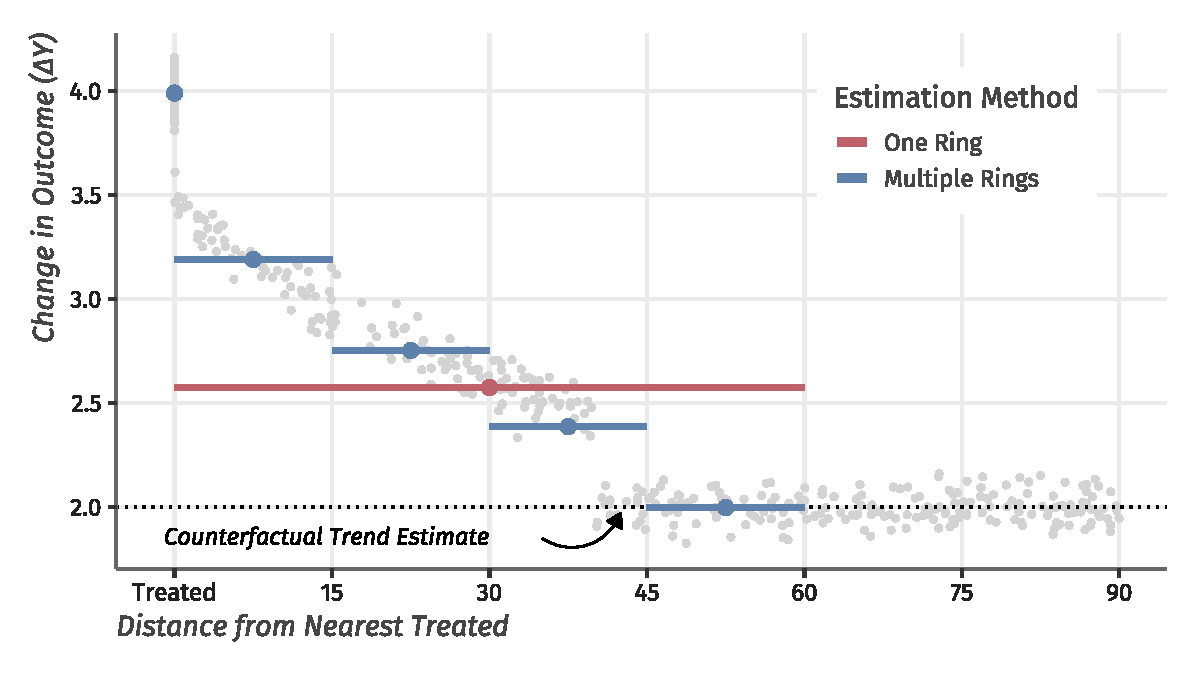
\includegraphics[width = \textwidth]{../../figures/figure-rings_v_within.pdf}

    {\footnotesize \textit{Notes:} The figure compares estimates of equation (\ref{eq:twfe_total}) with $S_i$ a ring of $(0, 60]$ miles from the nearest treated unit and of equation (\ref{eq:twfe_total_rings}) with rings for $(0,15], (15,30], (30,45], (45, 60]$ miles for a simulated set of data.}
\end{figure}

Panel (a) uses a single indicator for being between 0 and 60 miles from treatment and the difference between the bar and the estimated counterfactual trend is the estimated spillover effect which in this case is about 0.6. This number masks that units within the first 15 miles have a treatment effect of 1 or larger and units between 40 and 60 miles have 0 spillover effects. Figure (b) on the other hand uses 4 indicators for every 15 mile interval (0-15, 15-30, 30-45, and 45-60 miles). This improves on the estimate of a single ring in two ways. Multiple rings are better able to capture the evolution of spillover effects over distance. Furthermore, the ring that is included past the true maximum distance where spillover effects occur has a point estimate near zero. The rings method acts a semi-parametric estimator in the sense that as the number of rings increase and their width shrinks, the estimates would trace out the spillover effect function (subject to their being units outside of the rings). However, precision of estimates would decrease as the number of rings increase and therefore there is a bias-variance trade-off in the number and width of rings.\footnote{\citet{Clarke_2017} proposes a cross-validation technique for optimally choosing the number of rings and their techniques that uses the out-of-sample mean square prediction error as a way to estimate the bias-variance tradeoff. \citet{Butts_2021} provides a data-driven method to selecting rings under a more strict version of the parallel trends assumption.} 

One disadvantage of using a set of indicator for \textit{the nearest} treated unit is that some spillover effects are additive in the number of nearby treated units. In this case, summarizing exposure by the distance to the closest treated unit fails to capture important information on the location of other treated units and the coefficients on the ring indicators might be interpreted incorrectly. One potential solution is to count the number of treated units within each ring instead of creating indicators for nearest treated unit. This additive version of rings however no longer removes all bias from the direct effect of treatment unless the exposure mapping is correctly specified. Therefore, if spillover effects are expected to be additive in nature, seperate estimation of the direct effect and spillover effects would be the preferred method. 

% ------------------------------------------------------------------------------
\section{Application in Place-Based Policy Analysis}
\label{sec:tva}
% ------------------------------------------------------------------------------

To illustrate the importance of accounting for spatial spillovers in the estimation of treatment effects, I revisit the analysis of the Tennessee Valley Authority (TVA) in \citet{Kline_Moretti_2014}. The TVA program was a large-scale federal investment started in 1934 that focused on construction of dams and transportation canals in an attempt to modernize the Tennessee Valley's economy. By the end of WWII, the TVA became the largest single power supplier in the country and significantly lowered the cost of wholesale energy for factories.\footnote{More details on the program are found in \citet{Kline_Moretti_2014}. The effects on wholseale electricity are discussed in \citet{Kitchens_2014}.} With over \$20 Billion (in 2000 dollars) spent which is hundreds of dollars transferred per person in the Authority, the impacts are very likely to extend past the authority's borders. \citet{Kline_Moretti_2014} analyze a range of outcome variables, but for succinctness I use only (the log of) agricultural and manufacturing employment. Since the TVA primarily improved manufacturing industries through large-scale electrification, the authors predict that employment will grow in manufacturing and shrink in agricultural as workers switch to higher-paying manufacturing jobs. 

The analysis in \citet{Kline_Moretti_2014} begins by comparing changes in county-level outcomes from 1940 to either 1960 (short-run effects) or 2000 (long-run effects) between treated counties in the Authority and control counties outside. The primary specification is
\begin{equation}\label{eq:tva}
    y_{c, t} - y_{c, 1940} = \alpha + \text{TVA}_c \tau + X_{c, 1940} \gamma + (\varepsilon_{c, t} - \varepsilon_{c, 1940}),
\end{equation}
where $c$ denotes county, $\text{TVA}_c$ is an indicator variable for being in the Authority, $\text{Post}_t$ is an indicator for being in the post-period, and $y$ is a set of outcome variables (in logs).\footnote{The two-periods difference-in-differences regression is equivalent to a first-difference regression. The authors use an Oaxaca-Blinder estimator on the first differences and the results of \citet{Kline_2011} show that this estimator is equivalent to a weighted difference-in-differences estimate. Their estimator does not differ much from the standard difference-in-differences results since the weights are not that different from uniform weights.} Pre-treatment control variables, $X_{c,1940}$, are interacted with $\text{Post}_t$ to allow for places to be on different long-term trends.\footnote{See footnote 8 in \citet{Kline_Moretti_2014} for a full listing of control variables.} To improve the likelihood of the paralell trends assumption, they run a logistic regression to predict being in the TVA based on their set of control variables $X_{c,1940}$ and keep only observations in the top 75\% of predicted probability. The counties used in the sample are presented in Figure \ref{fig:tva_sample}. \citet{Kline_Moretti_2014} estimate (\ref{eq:tva}) to identify the `local effect' of the TVA -- what I am calling the `direct effect'. However, their point estimates compare, in part, changes in outcomes in TVA counties with changes in outcomes for neighboring counties that likely were impacted by the large-scale program. 

In the paper, the authors discuss the nature of spillovers that can occur. For agriculture employment, the authors claim that improved wages in the Authority will draw agriculture workers out of nearby counties. Hence they predict a negative spillover. For manufacturing, the sign is ambiguous. There could be positive spillovers if electrification brought cheap power and agglomeration economies to the neighboring areas. However, manufacturing could decline if firms chose to locate in the Authority that would have, in the absence of the program, decided to locate in nearby counties. My methodology will allow me to empirically test these predictions in the data and remove their bias from the treatment effect estimates. 

By comparing counties inside the Authroity to counties on the other side of the border, the authors likely underestimate the negative effect on agricultural employment while the bias in the manufacturing effect is theoretically ambiguous. The authors do recognize the problem of these comparisons and remove counties that share borders with the authority's, but due to the scale of the program, the spillovers are likely to extend further than this. Therefore, bias in their estimate will likely remain even after dropping contiguous counties. The estimation strategy I present keeps the observations near the TVA while controlling for spillover effects in a more rigorous manner.  

% Figure: TVA Effective Sample and Spillover Variables
\begin{figure}[tb!]
    \caption{TVA Effective Sample and Spillover Variables}
    \label{fig:tva_sample}

    {\centering
        \resizebox{\textwidth}{!}{
            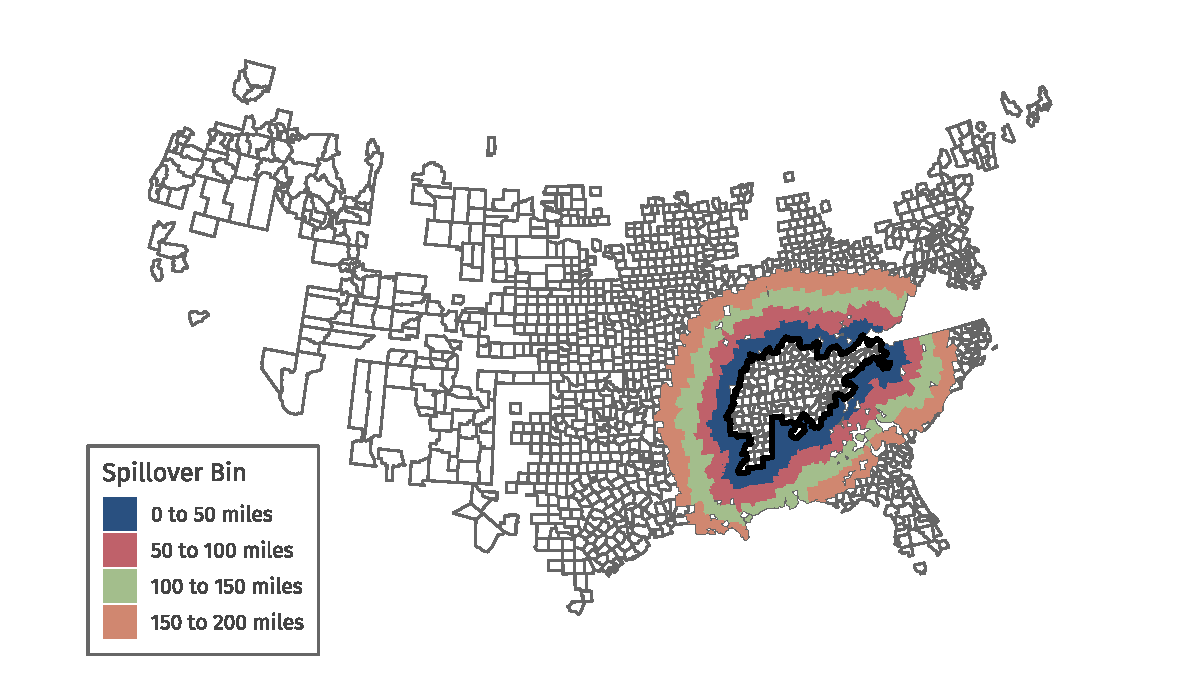
\includegraphics{../../figures/figure-tva-sample.pdf}
        } 
    }
    {\footnotesize \textit{Notes:} The above figure plots all the counties used in the estimation. Counties that fall within the distance intervals $\{ (0, 50], (50, 100], (100, 150], (150, 200] \}$ measured in miles are colored by their respective bin.} 
\end{figure}

I extend their analysis to control for spatial spillovers in the difference-in-differences specification. To parametrize the exposure mapping, I use a set of rings as described in Section \ref{sec:remove_bias}. Specifically, 
the specification with spillovers is given as follows:  
\begin{equation}\label{eq:tva_spillover}
    y_{i, t} - y_{i, 1940} = \alpha + \text{TVA}_i \tau + \sum_{d \in \text{Dist}} \text{Between}(d)\delta_d + X_{i, 1940} \beta + (\varepsilon_{i, t} - \varepsilon_{i, 1940}),
\end{equation} 
where $\text{Dist} = \{(0, 50], (50, 100], (100, 150], (150, 200]\}$ measured in miles and define $\text{Between}(d)$ as an indicator for being within the interval $d \in \text{Dist}$ away from the Authority and $t \in \{1960, 2000\}$. Figure \ref{fig:tva_sample} displays the four spillover variables by filling in each distance bin in a different color. The coefficients $\delta_d$ estimate the average spillover effect onto control units for each of these distance bins. From proposition \ref{thm:remove_bias}, $\hat{\tau}$ will be an unbiased estimate for the `local' effect so long as spillovers do not occur past 200 miles from the TVA.

The results of the long-run analysis from 1940 to 2000 are presented in Panel A Table \ref{tab:tva}. The first column lists which dependent variable (measured in logs) was used in the row. The following columns contain point estimates for $\tau$ and $\delta_d$'s in different specifications. The point estimates can be interpreted as decadel growth rates in outcomes. The column labeled difference-in-differences uses an ordinary least squares estimator for the specification without spillovers, equation (\ref{eq:tva}). This estimate finds a decline in agricultural employment of about $5.1\%$ per decade and an increase in manufacturing employment of about $5.6\%$ per decade. 

% Table: Effects of Tennessee Valley Authority on Decadel Growth
\begin{table}[!tb]
    \caption{Effects of Tennessee Valley Authority on Decadel Growth}
    \label{tab:tva}
    \renewcommand{\arraystretch}{1.1}

    \begin{adjustbox}{width = \textwidth, center}
        \begin{threeparttable}
            \begin{tabular}{@{} l c@{\extracolsep{20pt}}c@{\extracolsep{4pt}}cccc @{}}
                % Head
                \toprule

                & \multicolumn{1}{c}{\textbf{Diff-in-Diff}} & \multicolumn{5}{c}{\textbf{Diff-in-Diff with Spillovers}} \\ 
                \cmidrule{2-2} \cmidrule{3-7}
                & & & TVA between & TVA between & TVA between & TVA between \\ 
                & TVA & TVA & 0-50 mi. & 50-100 mi. & 100-150 mi. & 150-200 mi. \\ 
                \textit{Dependent Var.} & (1) & (2) & (3) & (4) & (5) & (6) \\
                
 
                % Body
                \toprule
                \multicolumn{7}{l}{\textbf{Panel A:} 1940-2000} \\
                \midrule
                
                 Population                  &    $0.0052$    &    $0.0053$    &    $-0.0040$   &    $-0.0212$   &    $-0.0077$   &    $-0.0053$   \\
                             &   $(0.0099)$   &   $(0.0090)$   &   $(0.0089)$   &   $(0.0179)$   &   $(0.0125)$   &   $(0.0123)$   \\
 Average manufacturing wage  &    $0.0064$    &  $0.0070^{**}$ &  $0.0075^{*}$  &    $0.0022$    &    $-0.0037$   &    $0.0023$    \\
                             &   $(0.0048)$   &   $(0.0030)$   &   $(0.0045)$   &   $(0.0047)$   &   $(0.0040)$   &   $(0.0047)$   \\
 Agricultural employment     & $-0.0561^{***}$& $-0.0514^{***}$& $-0.0678^{***}$& $-0.0310^{**}$ &    $-0.0112$   & $-0.0252^{***}$\\
                             &   $(0.0100)$   &   $(0.0087)$   &   $(0.0102)$   &   $(0.0123)$   &   $(0.0094)$   &   $(0.0084)$   \\
 Manufacturing employment    & $0.0606^{***}$ & $0.0560^{***}$ &  $0.0461^{**}$ &    $-0.0104$   &    $-0.0128$   &  $-0.0248^{*}$ \\
                             &   $(0.0170)$   &   $(0.0187)$   &   $(0.0210)$   &   $(0.0205)$   &   $(0.0257)$   &   $(0.0147)$   \\
 Value of farm production    &    $0.0024$    &    $-0.0060$   &    $-0.0184$   &    $-0.0188$   &    $-0.0101$   &    $-0.0266$   \\
                             &   $(0.0245)$   &   $(0.0269)$   &   $(0.0313)$   &   $(0.0252)$   &   $(0.0227)$   &   $(0.0176)$   \\
 Median family income        & $0.0219^{***}$ & $0.0191^{***}$ &  $0.0196^{**}$ &    $0.0056$    &    $-0.0062$   &    $-0.0011$   \\
                             &   $(0.0061)$   &   $(0.0067)$   &   $(0.0077)$   &   $(0.0079)$   &   $(0.0060)$   &   $(0.0032)$   \\
 Median housing value        &    $-0.0020$   &    $-0.0055$   &    $-0.0029$   &    $0.0039$    &    $0.0068$    &    $0.0006$    \\
                             &   $(0.0107)$   &   $(0.0091)$   &   $(0.0091)$   &   $(0.0163)$   &   $(0.0132)$   &   $(0.0063)$   \\


                \\ \toprule
                \multicolumn{7}{l}{\textbf{Panel B:} 1940-1960} \\
                \midrule 

                 Agricultural employment     & $0.0940^{***}$ &  $0.0856^{*}$  &    $-0.0062$   &    $-0.0042$   &    $-0.0303$   &    $-0.0039$   \\
                             &   $(0.0303)$   &   $(0.0498)$   &   $(0.0480)$   &   $(0.0480)$   &   $(0.0426)$   &   $(0.0359)$   \\
 Manufacturing employment    & $0.0894^{***}$ &  $0.0993^{**}$ &    $0.0228$    &    $0.0225$    &    $-0.0055$   &    $-0.0066$   \\
                             &   $(0.0324)$   &   $(0.0504)$   &   $(0.0496)$   &   $(0.0589)$   &   $(0.0384)$   &   $(0.0251)$   \\


                \\ \bottomrule
            \end{tabular}
            
            % Notes 
            \begin{tablenotes}\footnotesize
                \item \textit{Notes.} Each row corresponds to an outcome variable. Each cell is the point estimate and the standard error for the variable described in the column title. All standard errors are Conley standard errors with a correlation cutoff of 200 miles following \citet{Conley_1999}. The column labeled `Diff-in-Diff' estimates (\ref{eq:tva}) by OLS and is similar to the estimate reported in \citet{Kline_Moretti_2014}. The final four columns labeled `Diff-in-Diff with Spillovers' are estimates from (\ref{eq:tva_spillover}).
                
                \item $^{*} p< 0.1$; $^{**} p < 0.05$; $^{***} p < 0.01$.
            \end{tablenotes}
        \end{threeparttable}
    \end{adjustbox}
\end{table}


Turning to the specification that includes spillovers, equation (\ref{eq:tva_spillover}), column (2) contains a point estimate for $\tau$ and and columns (3)-(6) contain point estimates of the spillover effects $\delta_d$. For agricultural employment, the point estimates show there was a decline in agriculture employment in control units near the Authority. For control units between 0 and 50 miles, column (4) indicates a decline in agricultural employment of $3.7\%$ per decade. Between 50 and 100 miles the point estimate is $-1.6\%$ per decade, between 100 and 150 miles the point estimate is $-3\%$ per decade, and between 150 and 2000 miles the point estimate is $-1.6\%$ per decade. This is likely due to the fact that higher paying manufacturing jobs within the Authority drew farm-worker migrants from nearby counties. Because the spillovers onto the control counties is negative, the original difference-in-differences estimator was positively biased. The new point estimate indicates a decline of agricultural employment of about $7.4\%$ per decade compared to $5.1\%$ in the standard difference-in-difference specification. 

For manufacturing, our point estimates for spillovers are consistently negative, though imprecisely estimated in some columns. The spillover estimates suggest that neighboring counties experienced potentially negative spillover effects in the long-run. Since there are negative spillover effects present, the new point estimate in column (2) of $3.5\%$ is significantly smaller than the original estimate of $5.6\%$. The spillover estimates are evidence that in the long-run, urban shadow forces dominate the benefits of urban access. As you move away from the Tennessee Valley, the point estimates become more negative which suggest that the benefits of urban access vanish over distance faster than the costs of urban shadow.

To see how spillover effects from a large-scale place-based policy develop over time, Panel B in Table \ref{tab:tva} presents results for the effects of the Tennessee Valley in the short-run using outcome data in 1960. Unlike in the long-run, areas near the Tennessee Valley did not experience significant declines in agricultural employment in the short-run. Since our long-run analysis finds significant increases in high paying manufacturing employment in the Tennessee Valley, this result is consistent with long-run migration costs being lower than short-run costs.

For manufacturing, there are potentially positive increases in manufacturing employment within 100 miles of the Tennessee Valley authority and near zero effects between 100 and 200 miles. In the short-run, it appears that the effects of urban access and the cheap wholesale electricity dominated the effects of urban shadow. The effect of urban shadows can potentially be smaller in the short-run if operating firms are unlikely to relocate. Long-run effects can be larger as entrant firms change their location decision and operating firms are slowly replaced which is what the long-run spillover effect estimates suggest.

These results show that including spillovers in the estimation of direct treatment effects is potentially important and can lead to \emph{significant} differences in treatment effect estimates. Analysis of place-based policies that do not account for the fact that treatment effects can spillover beyond the borders of treated areas can potentially be biased. More, the spillover effects caused by place-based policies change over time as frictions can create delays in reoptimizing behavior. 

% ------------------------------------------------------------------------------
\subsection{Identification Strategies in Place-Based Policy Analysis}
% ------------------------------------------------------------------------------

More generally, my framework provides important insights into identification strategies when analysizing the effects of place-based policies. There are two ways I contribute. First, \citet{Baum-Snow_Ferreira_2015} recognize the problem of spatial spillovers causing problems in identification and point to aggregation of units as a way to alleviate to the problem (e.g. aggregating census tracts to metropolitan areas). However, this approach collapses the three seperate effects which might each be of interest into a singular aggregate effect. I have shown that all three effects of place-based policies can be estimated under very general assumptions about the spillovers. Therefore, the methods propose simple ways to estimate treatment effects with non-aggregated data.

Second, my framework provides insight for different identification strategies often used in the literature. Since place-based policies are targeted to specific distressed areas, comparison units are often hard to find. Researchers have developed many identification strategies to find comparison units that are facetimesimilar in terms of unobservables. First, researchers use border discontinuities to compare treated units to units just on the otehr side of the border. Other times, researchers compare approved applicants to narrowly rejected applicants. Both strategies aim to balance unobservables between treated and control units. A key difference in these identification strategies is the distance comparison units are from the treated area and therefore the former is more prone to bias due to spillovers than the latter.

For example, consider the analysis of the effects of federal Empowerment Zones. The federal Empowerment Zones are specially designated areas in high-unemployment areas. The program gives businesses located in the zone tax incentives and the goal of the program is to reduce unemployment and poverty. In the literature, there are a set of conflicting results with some papers suggesting that the Empowerment Zones do indeed reduce poverty rates and others finding near-zero effects.\footnote{See Table 1 of \citet{Neumark_Young_2019} for a summary of the various treatment effect estimates in the literature.} 

\citet{Busso_Gregory_Kline_2013} compare census tracts in Empowerment Zones to census tracts that qualified and were rejected from the program. The rejected tracts are not typically geographically near accepted Empowerment Zones and they find large significant reductions in poverty rates. Meanwhile, \citet{Neumark_Kolko_2010} compare census tracts in Empowerment Zones to census tracts within 1,000 feet of the Zone. These control counties are likely the ones that experience the largest spillover effects and they find near-zero effects on poverty. 

My framework can reconcile both of these results. If census tracts just outside the Empowerment Zones also benefit from the policy, then the estimates of \citet{Neumark_Kolko_2010} are attenuated towards zero. These two identification strategies of using rejected applicants or using bordering units as the control group are very common in the urban literature more generally \citep{Baum-Snow_Ferreira_2015}. My paper suggests that the former is the preferred strategy if spillovers occur onto nearby control units. Identification strategies that rely on geographically close control units as having similar unobservables should be used cautiously. If treatment effects spillover treatment border, then estimated treatment effects can be biased.



% ------------------------------------------------------------------------------
\section{Estimating Event Study with Spillovers}
\label{sec:event_study}
% ------------------------------------------------------------------------------

The intuition from how spillovers cause biases in estimates of the direct effect of treatment extend into the setting where there is staggered adoption in treatment. When treatment turns on for different units at different times, two-way fixed effect estimates can be viewed as a weighted sum of $2 \times 2$ difference-in-differences estimates.\footnote{Various forms for these weights are described in \citet{Goodman-Bacon_2018}, \citet{Sun_Abraham_2020}, and \citet{deChaisemartin_DHaultfoeuille_2019}. I do not recharacterize the weights in this article and guide interested readers to the source articles themselves.} Therefore the bias terms will be an identically weighted sum of the bias term(s) from the $2 \times 2$ estimates, assuming that the parallel counterfactual trends assumption (\ref{assumption:parallel}) holds. However, since weights on some of the $2 \times 2$ estimates can be negative, the sign of the spillover effects do not determine the sign of the weighted average of the spillover effects. This makes the bias from spillovers much more difficult to sign. 

In order to estimate treatment effects in the presence of spatial spillovers and staggered treatment timing, I will propose an estimation strategy that follows the `imputation-based' approach proposed in concurrent work by \citet{Gardner_2021} and \citet{Borusyak_Jaravel_Spiess_2021} while incorporating spillovers directly into estimation. I assume I observe an independent and identically distributed panel for units $i$ and periods $t$. The imputation-based method relies on a model-based assumption for untreated/unexposed units to formalize parallel trends:
\begin{assumption}[Parallel Counterfactual Trends (Staggered)]\label{assumption:parallel_staggered}
    For all units and all periods, the untreated and unexposed outcome is given by
    \begin{equation}\label{eq:y0_staggered}
        Y_{it}(0, \vec{0}) = \mu_i + \lambda_t + \varepsilon_{it},
    \end{equation}
    where $\expec{\varepsilon_{it}} = 0$, $\mu_i$ and $\lambda_t$ are non-stochastic unit and time fixed effects.
\end{assumption}
This formalizes parallel trend by imposing that there is a common time-trend in the absence of treatment, $\lambda_t$. Note that this does not impose any structure on the effects of treatment and exposure $(D_{it}, h(\vec{D},i))$. I also assume that units do not have any anticipatory effects before treatment starts:
\begin{assumption}[No Anticipation (Staggered)]\label{assumption:no-anticipation_staggered}
    For all observations with $D_{it} = 0$ and $h(\vec{D}, i) = 0$, $Y_{it}(D, \vec{h}) = Y_{it}(0,0)$ for all values of $D$ and $\vec{h}$.
\end{assumption}

With a model for $Y_{it}(0, \vec{0})$, treatment effects for individual $i$ and time $t$ under treatment status $D_{it}$ and exposure $h(\vec{D}, i)$ are given by $\tau_{it}(D_{it}, h(\vec{D}, i)) = Y_{it}(D_{it}, h(\vec{D}, i)) - Y_{it}(0, \vec{0})$. Then, the total effect and the direct effect are formed similar to above:
\[
    \tau_{\text{total}} \equiv \expec{ \tau_{it}(1, h(\vec{D}, i)) \ \vert \ D_{it} = 1} \text{ and }
    \tau_{\text{direct}} \equiv \expec{ \tau_{it}(1, 0) \ \vert \ D_{it} = 1, h(\vec{D},i) = \vec{0}}.
\]
However, it is also common in event-study analyses to allow heterogeneity in effects by the number of years that a unit experiences treatment. Let $K_{it}$ denote the number of years since treatment turns on (-1 for year prior, 0 for intial year, and so on). Then we can define dummy variables $D_{it}^k \equiv D_it \one_{K_{it} = k}$ and estimate average total effects for each relative period: 
\[
    \tau_{\text{total}}^k \equiv \expec{ \tau_{it}(1, h(\vec{D}, i)) \ \vert \ D_{it}^k = 1},
\]
and similarly for the direct effect.

Estimation of $\tau_{it}$ is the difference between the observed $Y_{it}$ and the unobserved outcome $Y_{it}(0, \vec{0})$ which we will estimate using observations with $D_{it} = 0$ and $h(\vec{D}, 0) = \vec{0}$. Similar to the previous section, under assumption (\ref{assumption:local}) we define $S_{it}$ to be an indicator equal to one if in period $t$, unit $i$ is within $\bar{d}$ distance from the nearest treated unit. Following the procedure laid out in \citet{Gardner_2021}, I propose a modified version of the two-stage difference-in-differences estimator: 

\begin{enumerate}
    \item Estimate $Y_{it} = \mu_i + \lambda_t + u_{it}$ for observations with $D_{it} = 0$ and $S_{it} = 0$ to estimate the common trend $\lambda_t$ and unit fixed effects $\mu_i$. For all observations, residualize $\tilde{Y}_{it} \equiv Y_{it} - \hat{\mu}_i - \hat{\lambda}_t$ which is our estimate for $\tau_{it}$.
    
    \item Regress $\tilde{Y}_{it}$ on treatment and spillover dummy variables (discussed in table (\ref{tab:second_stage})).
\end{enumerate}

The first stage uses untreated and unexposed outcomes to consistently estimate the model (\ref{eq:y0_staggered}). Then, $\tilde{Y}_{it}$ will serve as an estimate for $\tau_{it}$. The second stage regression can be used to estimate averages of $\tau_{it}$ for different groups depending on the parameters of interest. This is equivalent to regressing the residual $\tilde{Y}_{it}$ on dummy variable(s). Table \ref{tab:second_stage} provides examples of treatment effects of interest and corresponding dummy variables to include. 

% Table: Bias from Misspecification of Spillovers
\begin{table}[!tb]
    \caption{Second Stage Variables}
    \label{tab:second_stage}

    \centering
    \begin{threeparttable}
        \begin{tabular}{@{} *{2}{l} @{}}
            % Head
            \toprule
            \textbf{Estimand} & \textbf{Included Variables} \\

            % Body
            \midrule
            Total Effect & $D_{it}$ \\
            Total Effect (Event Study) & $D_{it}^k$ dummies \\
            Direct Effect & $D_{it}(1 - S_{it})$ \\
            Direct Effect (Event Study) & $D_{it}^k(1 - S_{it})$ dummies \\
            Spillover Effect on Control & $S_{it}(1 - D_{it})$ or $\text{Ring}_{it}(1-D_{it})$ \\
            Spillover Effect on Control (Event Study) & $S_{it}^k(1 - D_{it})$ or $\text{Ring}_{it}^k(1-D_{it})$ \\
            \bottomrule
        \end{tabular}
    \end{threeparttable}

\end{table}

As discussed in \citet{Gardner_2021}, inference must account for the fact that the regressand in the second stage is estimated in step 1. \citet{Gardner_2021} propose reframing the two-stage process as a two-stage GMM estimator and discusses how to perform valid inference in this setting. This procedure is implemented in the R/Stata package \texttt{did2s} \citep{did2s}.



% ------------------------------------------------------------------------------
\subsection{Application on Community Health Centers}\label{sec:chc}
% ------------------------------------------------------------------------------

As an application of the above methods, I extend the analysis of \citet{Bailey_Goodman_Bacon_2015}. The authors study the creation of federal community health centers between 1965 and 1974 that provided \textit{primary} care to low-income communities. They test the hypothesis if access to low/no- cost health care services decreased mortality rates on the treated population. To answer this question, the authors use a common event-study framework to compare outcomes in treated counties to all other US counties by estimating the following specification 
\begin{equation}\label{eq:chc_es}
    Y_{it} = \theta_i + X_{it} \beta + \sum_{k = -7}^{-2} \pi_y D_{it}^k + \sum_{k = 0}^{15} \tau_{y} D_{it}^k + \varepsilon_{it},
\end{equation}
where $D_i^k$ is the typical `event study' indicator for being treated for $k$ years, $\theta_i$ is county fixed effects, and $X_{it}$ contains a set of controls.\footnote{Controls include 1960 county characteristic trends, state-year fixed effects, and urban-group fixed effects. A full list can be found on page 1080 of \citet{Bailey_Goodman_Bacon_2015}.} The coefficents $\pi_y$ can be interpreted as tests of parallel pre-trends and $\tau_y$ can be interepreted as the treatment effect of a community health center $y$ years after establishment. In years following the establishment of the community health centers, the authors find a reduction of between 15-30 deaths per 100,000 residents compared to a baseline adjusted mortality rate of 929 deaths per 100,000 residents. 

% Figure: Direct and Spillover Effects of Community Health Centers
\begin{figure}[tb!]
    \caption{Direct and Spillover Effects of Community Health Centers}
    \label{fig:chc_es_spill}
        
    {\centering
        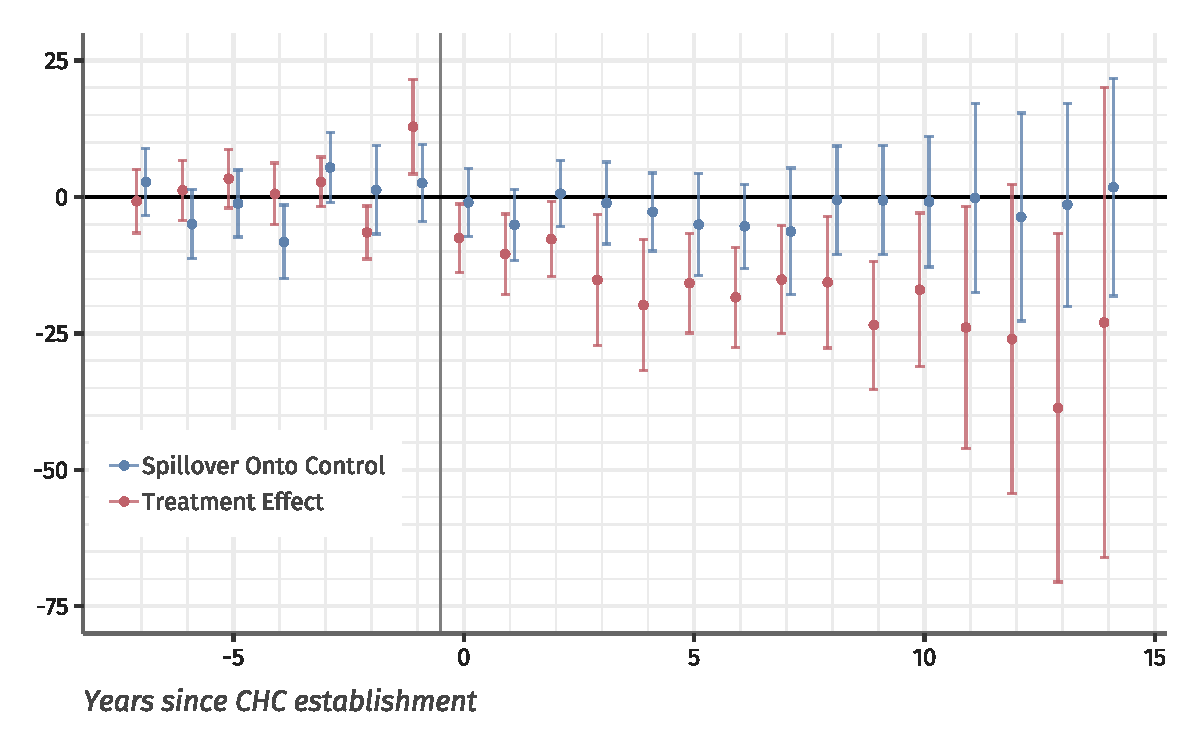
\includegraphics[width=\textwidth]{../../figures/figure-chc-es_combined.pdf}
    }
    {\footnotesize
        \textit{Notes:} This figure plots event study estimates for the total effect and the spillover effect on control units within 25 miles of treatment at different periods relative to establishment year. The estimates are generated using the `did2s' package \citep{did2s}. 
    }
\end{figure}


There are theoretical reasons to think spillovers may or may not exist in this context. On the one hand, individuals outside the county can potentially travel to the community health centers to receive care. This would create a negative spillover effect on mortality rates in nearby counties which would bias their estimates towards zero. On the other hand, \citet{Bailey_Goodman_Bacon_2015} document evidence that their estimated effects are not due to emergency but rather primary care services. In this case, it is less likely low-income individuals would travel very far to receive primary care and hence the spillover effects is potentially near zero. My methodology can provide an answer to the question of how far do individuals travel for low/no -cost primary care.

As in the method detailed above, I use the subsample of counties that do not receive a community health center and use an indicator for being within 25 miles of a treated county as the treatment variable. Then, I follow \citet{Callaway_SantAnna_2020} in estimating event-study coefficients. The results are presented in Figure \ref{fig:chc_es_spill}. The confidence intervals labeled with circles represent point estimates for the average spillover effect on control units within 25 miles. No spillover effect is estimated to be significantly different from zero which suggests that the effects of community health centers are very local. Since there are near zero spillover effects, the direct effect estimates marked in Figure \ref{fig:chc_es_spill} as diamonds maintain the same shape as the author's original estimates with estimates between 15-30 fewer deaths per 100,000 persons. 

The spillover effects results provide evidence that low-income individuals will not travel far to receive primary care. Practically, this suggests that community health centers should be targeted to be as accessible as possible for poor individuals as they are unable to travel far to access the services. 







% ------------------------------------------------------------------------------
\section{Discussion}
\label{sec:conclusion}
% ------------------------------------------------------------------------------

This paper has considered the common environment where treatment is assigned via administrative boundary while the effects of treatment spread across these borders. In this context, difference-in-differences estimation will identify a combination of the direct effect of treatment and two additional terms resulting from spillovers. I use a potential outcomes framework that formalizes spillovers to improve upon ad-hoc estimation strategies by proposing a new estimation strategy that is robust to more forms of spillovers. In particular, I find that specifications with an indicator for being ``close to'' treated units interacted with treatment status will remove all bias in the direct effect estimate so long as all units affected by spillovers are contained in the indicator. More, I show that a set of concentric `rings' are the best at capturing the spatial structure of spillovers. When estimating spillover effects themselves, I find that it is important to correctly identify is spillovers are additive or non-additive in the number of nearby treated units.  

Then, I show that in settings with spatial spillovers, estimates can change significantly. In particular, place-based interventions change the nature of agglomeration in the local and surrounding area--that is cause spillovers--local effects of these policies can be misestimated without controlling for general equilibrium effects. I also show the importance of considering spillovers in weighing the pros and cons of various identificatin strategies. Identification strategies based on geographic continuity of unobservables can magnify the bias from spillovers as they restrict the compairson group to observations experiencing the largest spillover effects.




% \section*{Acknowledgements}

% I am grateful to Taylor Jaworski, Adam McCloskey, Damian Clarke, Daniel Kaffine, Tania Barham, Alexander Bentz, James Flynn, Brach Champion, Hannah Denker, and participants of the Western Economics Association Conference and the CU Boulder Labor Economics Seminar for helpful feedback.


% ------------------------------------------------------------------------------
\setlength{\bibsep}{0.0pt}
\bibliography{references.bib}
% ------------------------------------------------------------------------------


% ------------------------------------------------------------------------------
\appendix 
% ------------------------------------------------------------------------------

% ------------------------------------------------------------------------------
\section{Proofs}
\label{sec:proofs}
% ------------------------------------------------------------------------------

% ------------------------------------------------------------------------------
\subsection{Proof of Theorem \ref{thm:bias}}
% ------------------------------------------------------------------------------

\begin{align*}
    &\underbrace{\expec{Y_{i1} - Y_{i0} \mid D_i = 1 } - \expec{Y_{i1} - Y_{i0} \mid D_i = 0 }}_{\text{Difference-in-Differences}} \\
    &= \expec{Y_{i1}(1, h(\vec{D}, i)) - Y_{i0}(0, \vec{0})  \mid D_i = 1 } - \expec{Y_{i1}(0, h(\vec{D}, i)) - Y_{i0}(0, \vec{0}) \mid D_i = 0 } \\
    &= \expec{Y_{i1}(1, h(\vec{D}, i)) - Y_{i0}(0, \vec{0})  \mid D_i = 1 } \\
    &\quad\quad - \expec{Y_{i1}(0, h(\vec{D}, i)) + Y_{i1}(0, \vec{0}) - Y_{i1}(0, \vec{0}) - Y_{i0}(0, \vec{0}) \mid D_i = 0 } \\
    &= \expec{Y_{i1}(1, h(\vec{D}, i)) - Y_{i0}(0, \vec{0})  \mid D_i = 1 } - \expec{Y_{i1}(0, \vec{0}) - Y_{i0}(0, \vec{0}) \mid D_i = 0} \\ 
    &\quad\quad - \expec{Y_{i1}(0, h(\vec{D}, i)) - Y_{i1}(0, \vec{0})\mid D_i = 0} \\ 
    &= \expec{Y_{i1}(1, h(\vec{D}, i)) - Y_{i0}(0, \vec{0})  \mid D_i = 1 } - \expec{Y_{i1}(0, \vec{0}) - Y_{i0}(0, \vec{0}) \mid D_i = 1} \\
    &\quad\quad - \expec{Y_{i1}(0, h(\vec{D}, i)) - Y_{i1}(0, \vec{0})\mid D_i = 0} \\  
    &= \expec{Y_{i1}(1, h(\vec{D}, i)) - Y_{i0}(0, \vec{0}) - Y_{i1}(0, \vec{0}) + Y_{i0}(0, \vec{0})\mid D_i = 1 } \\
    &\quad\quad - \expec{Y_{i1}(0, h(\vec{D}, i)) - Y_{i1}(0, \vec{0})\mid D_i = 0}\\
    &= \expec{Y_{i1}(1, h(\vec{D}, i)) - Y_{i1}(0, \vec{0}) \mid D_i = 1 } - \expec{Y_{i1}(0, h(\vec{D}, i)) - Y_{i1}(0, \vec{0})\mid D_i = 0}\\
    &= \expec{Y_{i1}(1, h(\vec{D}, i)) + Y_{i1}(1, \vec{0}) - Y_{i1}(1, \vec{0}) - Y_{i1}(0, \vec{0})\mid D_i = 1 } \\
    &\quad\quad - \expec{Y_{i1}(0, h(\vec{D}, i)) - Y_{i1}(0, \vec{0})\mid D_i = 0} \\
    &= \expec{Y_{i1}(1, \vec{0}) - Y_{i1}(0, \vec{0}) \mid D_i = 1} + \expec{Y_{i1}(1, h(\vec{D}, i)) - Y_{i1}(1, \vec{0}) \mid D_i = 1} \\
    &\quad\quad - \expec{Y_{i1}(0, h(\vec{D}, i)) - Y_{i1}(0, \vec{0}) \mid D_i = 0} \\
    &\equiv \tau_{\text{direct}} + \tau_{\text{spill}}(1) - \tau_{\text{spill}}(0) = \tau_{\text{total}} - \tau_{\text{spill}}(0) \\
\end{align*}



% ------------------------------------------------------------------------------
\subsection{Proof of Theorem \ref{thm:remove_bias}}
% ------------------------------------------------------------------------------

For part (i):

\begin{align*}
    &\expec{Y_{i1} - Y_{i0} \ \mid \ D_i = 1} - \expec{Y_{i1} - Y_{i0} \ \mid \ D_i = 0, S_i = 0} \\
    &\quad\quad= \expec{Y_{i1}(1, h(\vec{D},i)) - Y_{i0}(0,0) \ \mid \ D_i = 1} - \expec{Y_{i1}(0, 0) - Y_{i0}(0,0) \ \mid \ D_i = 0} \\
    &\quad\quad= \expec{Y_{i1}(1, h(\vec{D},i)) - Y_{i0}(0,0) \ \mid \ D_i = 1} - \expec{Y_{i1}(0, 0) - Y_{i0}(0,0) \ \mid \ D_i = 1} \\
    &\quad\quad= \expec{Y_{i1}(1, h(\vec{D},i)) - Y_{i0}(0,0) - Y_{i1}(0, 0) + Y_{i0}(0,0) \ \mid \ D_i = 1} \\
    &\quad\quad= \expec{Y_{i1}(1, h(\vec{D},i)) - Y_{i1}(0, 0) \ \mid \ D_i = 1} \\
    &\quad\quad\equiv \tau_{\text{total}},
\end{align*}
where the first equality comes from the fact that $S_i = 0$, the second equality from parallel trends assumption (\ref{assumption:parallel-mod}), and the last by definition of the total effect.

Similarly, for part (ii):

\begin{align*}
    &\expec{Y_{i1} - Y_{i0} \ \mid \ D_i = 1, S_i = 0} - \expec{Y_{i1} - Y_{i0} \ \mid \ D_i = 0, S_i = 0} \\
    &\quad\quad= \expec{Y_{i1}(1, 0) - Y_{i0}(0,0) \ \mid \ D_i = 1, S_i = 0} - \expec{Y_{i1}(0, 0) - Y_{i0}(0,0) \ \mid \ D_i = 0, S_i = 0} \\
    &\quad\quad= \expec{Y_{i1}(1, 0) - Y_{i0}(0,0) \ \mid \ D_i = 1, S_i = 0} - \expec{Y_{i1}(0, 0) - Y_{i0}(0,0) \ \mid \ D_i = 1, S_i = 0} \\
    &\quad\quad= \expec{Y_{i1}(1, 0) - Y_{i0}(0,0) - Y_{i1}(0, 0) + Y_{i0}(0,0) \ \mid \ D_i = 1, S_i = 0} \\
    &\quad\quad= \expec{Y_{i1}(1, 0) - Y_{i1}(0, 0) \ \mid \ D_i = 1, S_i = 0} \\
    &\quad\quad= \expec{Y_{i1}(1, 0) - Y_{i1}(0, 0) \ \mid \ D_i = 1} \\
    &\quad\quad\equiv \tau_{\text{direct}},
\end{align*}
where the first equality comes from the fact that $S_i = 0$, the second equality from parallel trends assumption (\ref{assumption:parallel-mod}) and 
the second to last equality follows from assumption (\ref{assumption:homogenous-direct}).



% ------------------------------------------------------------------------------
\section{Monte Carlo Simulations}
% ------------------------------------------------------------------------------

% ------------------------------------------------------------------------------
\subsection{Bias Under Misspecification of Spillovers}
% ------------------------------------------------------------------------------

To illustrate the above discussion, I turn to a set of Monte Carlo simulations. The first exercise is to consider a set of different data generating processes and see how well estimates of the direct effect perform when controlling for spillovers using potentially misspecified exposure mappings. In the general form, I generate data with unit and time fixed effects and an error term that is uncorrelated with $D_{it}$ for many different exposure mappings $h(\vec{D}, i)$. I generate data for unit $i$ is a US county at time $t \in \{1, \dots, 20\}$ using the following data-generating process:
\begin{equation}\label{eq:dgp_general}
    y_{it} = \lambda_t + \mu_i + 2 D_{it} + \beta_{\text{spill, control}} (1-D_{it}) h(\vec{D}, i) + \varepsilon_{it},
\end{equation}
where $\lambda_t \sim N(0.2t, 0.1^2)$ and $\mu_i \sim N(6, 2^2)$ respectively and the error term is IID and distributed as $\varepsilon_{it} \sim N(0, 2^2)$. 

For simplicity, I also remove spillovers onto treated units, but the results of which specifications perform best in the simulation are the same. In order to keep the magnitude of bias constant across specifications, I normalize the average spillover magnitude to be equal across specifications.\footnote{This results in a constant bias for TWFE estimates across data-generating processes.} For each true data-generating process, I estimate (\ref{eq:dgp_general}) with the correct spillover and misspecified alternatives $\tilde{h}(\vec{D}, i)$. 

The set of spillover specifications included in the data-generating process are `Within $40/80$mi.' which equals 1 if the counties' center of population is within $40/80$ miles to a treated county's center of population. `Within $40/80$mi. (Additive)' is the number of treated county's within $40/80$ miles of the control county. `Decay' is given by $\max_j D_j e^{-0.02 d(i,j)} * 1(d(i,j) < 80)$ and `Decay (Additive)' is given by $\sum_{j \neq i} D_j \exp^{-0.02 d(i,j)}$.

The last set of spillover specifications is commonly used in the literature as a semi-parametric estimator and are referred to as `Rings'. These consist of a set of indicators for falling within distance bins from the nearest treated unit (e.g. indicators for being between 0-20, 20-40, 40-60, and 60-80 miles to closest treated unit). The last specification is an additive version of `Rings' which is the number of treated units within each distance bin. This maintains a lot of the intuitive advantages of the `Rings' specification but parameterizes the spillovers to be additive in the number of nearby treated units. The advantage of this, as seen below, is enhanced performance of estimating spillover effects that are additive in nature. However, if the true specification is non-additive, then the additive specification no longer will remove all the bias from the direct effect estimate.

% Table: Bias from Misspecification of Spillovers
\begin{table}[!tb]
    \caption{Bias from Misspecification of Spillovers}
    \label{tab:misspecification}
    \renewcommand\arraystretch{1}

    \begin{adjustbox}{width = 1.1\textwidth, center}
        \begin{threeparttable}
            \begin{tabular}{@{} l *{6}{d{2.4}} @{}}
                % Head
                \toprule
                & \multicolumn{6}{c}{Data-Generating Process} \\
                \cmidrule{2-7}

                & \mcl{\textbf{Within 40mi}} & \mcl{\textbf{Within 80mi}} & \mcl{\textbf{Within 40mi.}} & \mcl{\textbf{Within 80mi.}} & \mcl{\textbf{Decay}} & \mcl{\textbf{Decay}} \\
                Specification & & & \mcl{\textbf{(Additive)}} & \mcl{\textbf{(Additive)}} & & \mcl{\textbf{(Additive)}} \\
 
                % Body
                \midrule
                
                
TWFE (No Spillovers)                                   & 0.263   & 0.263   & 0.263   & 0.263   & 0.263   & 0.263   \\
                                                       & [0.091] & [0.091] & [0.091] & [0.091] & [0.091] & [0.091] \\
Within 40mi.                                           & 0.000   & 0.219   & 0.164   & 0.000   & 0.182   & 0.149   \\
                                                       & [0.022] & [0.070] & [0.049] & [0.022] & [0.055] & [0.044] \\
Within 80mi.                                           & 0.000   & 0.000   & 0.000   & 0.000   & 0.000   & 0.000   \\
                                                       & [0.024] & [0.024] & [0.024] & [0.024] & [0.024] & [0.024] \\
Within 40mi. (Additive)                                & 0.049   & 0.227   & 0.179   & -0.001  & 0.183   & 0.149   \\
                                                       & [0.025] & [0.074] & [0.054] & [0.022] & [0.055] & [0.044] \\
Within 80mi. (Additive)                                & 0.043   & 0.142   & 0.107   & -0.004  & -0.001  & -0.003  \\
                                                       & [0.025] & [0.043] & [0.034] & [0.023] & [0.023] & [0.023] \\
Decay                                                  & -0.151  & 0.079   & 0.000   & -0.166  & 0.024   & -0.024  \\
                                                       & [0.046] & [0.030] & [0.024] & [0.051] & [0.024] & [0.024] \\
Decay (Additive)                                       & -0.015  & 0.155   & 0.095   & -0.077  & 0.026   & -0.001  \\
                                                       & [0.023] & [0.047] & [0.032] & [0.029] & [0.024] & [0.023] \\
Rings (0-20, 20-30, 30-40)                             & 0.000   & 0.219   & 0.164   & 0.000   & 0.182   & 0.149   \\
                                                       & [0.022] & [0.070] & [0.049] & [0.022] & [0.055] & [0.044] \\
Rings (0-20, 20-30, 30-40, 40-60, 60-80)               & 0.000   & 0.000   & 0.000   & 0.000   & 0.000   & 0.000   \\
                                                       & [0.024] & [0.024] & [0.024] & [0.024] & [0.024] & [0.024] \\
Rings (0-20, 20-30, 30-40, 40-60, 60-80) (Additive)    & 0.044   & 0.142   & 0.108   & -0.001  & -0.001  & -0.001  \\
                                                       & [0.025] & [0.043] & [0.035] & [0.023] & [0.023] & [0.023] 
                
                \\ \bottomrule
            \end{tabular}
            
            % Notes 
            \begin{tablenotes}\footnotesize
                \item \textit{Notes.} Each cell corresponds to the results from 1000 simulations of the data generating process specified by the column header and estimated by equation (\ref{eq:dgp_general}) with $\tilde{h}(\vec{D},i)$ given by the row label. The non-bracketed number represents the mean bias from the simulations and the bracketed number represents the mean square error given by $\sum_{i = 1}^n \frac{(\hat{\tau}_i - \tau_0)^2}{n}$
            \end{tablenotes}
        \end{threeparttable}
    \end{adjustbox}
\end{table}

The results of the simulations are produced in Table \ref{tab:misspecification}. For each entry in the table, the column label corresponds to the true exposure mapping used in the data-generating process and the row label corresponds to the exposure mapping, $\tilde{h}(\vec{D}, i)$, used in estimation.  The corresponding cell gives the mean bias from estimating equation (\ref{eq:dgp_general}) with the $\tilde{h}(\vec{D}, i)$ given by the row. The bracketed number below the mean bias is the mean-squared error of the estimate which is given by $\sum_{i=1}^n \frac{(\hat{\tau}_{i,\text{direct}} - \tau_0)^2}{n}$. The mean squared error combines the square of the bias term, the variance of the estimator, and the variance of the error term which does not depend on the equation specification. This measure gives a good sense of the trade-off with whether decreasing bias comes at the cost of increasing the variance of the estimator.

The first thing to note is that all specifications remove a large portion of the bias relative to traditional two-way fixed effect estimate and lower the mean-squared error. In particular, correctly specifying the data-generating process removes almost all the bias in the direct effect estimate and greatly lowers the mean-squared error. The second result is that both the non-additive `Rings' and the `Within' specification perform best among all the misspecified spillovers in terms of removing bias, so long as they are wide enough to capture all the spillovers (see Proposition \ref{thm:remove_bias}). These specifications do so without increasing the variance of the estimator relative to the true specification. However, if the indicator is not wide enough as is the case with Within 40mi. for the 80mi. data-generating process, bias remains in the estimates. Therefore, if researchers are primarily interested in identifying the direct effect, then either `Rings' or `Within' specifications with a large cutoff distance are preferred.

% ------------------------------------------------------------------------------
\subsection{Spillover Effect Estimation}
% ------------------------------------------------------------------------------

Now, I turn to analyzing how the specifications perform at estimating the spillover effects themselves. For the next table, I predict the spillover effect for each control unit from the point estimates on $\tilde{h}(\vec{D}, i)$. Then as a measure for how well spillovers are estimated, I will calculate one minus the mean squared prediction error normalized by the sum of squared spillovers (for comparison across data-generating processes), 
\begin{equation}\label{eq:mspe}
    1 - \frac{\sum_{i: D_i = 0} (\beta_{\text{spill, control}} h(\vec{D}, i) - \hat{\beta}_{\text{spill, control}} \tilde{h}(\vec{D}, i))^2}{\sum_{i: D_i = 0} (\beta_{\text{spill, control}} h(\vec{D}, i))^2}.
\end{equation} 
This will produce a percentage of spillovers that are explained by the specification, so numbers closer to $100\%$ represent better modelling of the spillovers. 

% Table: Percent of Spillovers Predicted by Specification
\begin{table}[!tb]
    \caption{Percent of Spillovers Predicted by Specification}
    \label{tab:misspecification_mspe}

    \begin{adjustbox}{width = 1.1\textwidth, center}
        \begin{threeparttable}
            \begin{tabular}{@{} l *{6}{d{2.2}} @{}}
                % Head
                \toprule
                & \multicolumn{6}{c}{Data-Generating Process} \\
                \cmidrule{2-7}

                & \mcl{\textbf{Within 40mi}} & \mcl{\textbf{Within 80mi}} & \mcl{\textbf{Within 40mi.}} & \mcl{\textbf{Within 80mi.}} & \mcl{\textbf{Decay}} & \mcl{\textbf{Decay}} \\
                Specification & & & \mcl{\textbf{(Additive)}} & \mcl{\textbf{(Additive)}} & & \mcl{\textbf{(Additive)}} \\
 
                % Body
                \midrule
                
                
                TWFE (No Spillovers) & $0.0\%$ & $0.0\%$ & $0.0\%$ & $0.0\%$ & $0.0\%$ & $0.0\%$ \\ 
Within 40mi. & $99.3\%$ & $25.0\%$ & $58.8\%$ & $85.4\%$ & $38.4\%$ & $55.6\%$ \\ 
Within 80mi. & $39.5\%$ & $96.4\%$ & $85.7\%$ & $33.9\%$ & $71.5\%$ & $67.6\%$ \\ 
Within 40mi. (Additive) & $85.1\%$ & $20.5\%$ & $51.4\%$ & $99.5\%$ & $40.5\%$ & $60.6\%$ \\ 
Within 80mi. (Additive) & $45.5\%$ & $61.0\%$ & $70.5\%$ & $47.2\%$ & $98.3\%$ & $93.5\%$ \\ 
Decay & $60.1\%$ & $81.8\%$ & $97.4\%$ & $52.7\%$ & $75.5\%$ & $81.9\%$ \\ 
Decay (Additive) & $60.4\%$ & $55.6\%$ & $78.0\%$ & $63.8\%$ & $93.2\%$ & $98.4\%$ \\ 
Rings (0-20, 20-30, 30-40) & $98.4\%$ & $22.8\%$ & $58.2\%$ & $85.7\%$ & $37.1\%$ & $55.8\%$ \\ 
Rings (0-20, 20-30, 30-40, 40-60, 60-80) & $96.7\%$ & $91.9\%$ & $92.1\%$ & $84.2\%$ & $72.7\%$ & $78.4\%$ \\ 
Rings (0-20, 20-30, 30-40, 40-60, 60-80) (Additive) & $83.3\%$ & $56.6\%$ & $72.7\%$ & $97.6\%$ & $94.9\%$ & $94.8\%$
                
                \\ \bottomrule
            \end{tabular}
            
            % Notes 
            \begin{tablenotes}\footnotesize
                \item \textit{Notes.} Each cell corresponds to the results from 1000 simulations of the data generating process specified by the column header and estimated by equation (\ref{eq:dgp_general}) with $\tilde{h}(\vec{D},i)$ given by the row label. The number corresponds to the mean square prediction error of the spillover effect for each control unit normalized by the total variance of spillover effects, given by Equation \ref{eq:mspe}.
            \end{tablenotes}
        \end{threeparttable}
    \end{adjustbox}
\end{table}

Results of this exercise are presented in Table \ref{tab:misspecification_mspe}. For each specification, correctly specifying the spillovers produces the best estimates for spillovers as expected. Among misspecified exposure mapping, `Rings' that are large enough to caputre all the spillovers perform better than all other specifications in all non-additive data-generating processes. On the other hand, when the spillovers are additive, the predicted spillovers from the non-additive ring specifications do not as accurately measure these spillovers as they did before.\footnote{Although the non-additive Rings do estimate between 70\% and 80\% of the spillover effects while maintaining complete removal of bias.} Non-additvie specifciations perform somewhat poorly at estimating spillovers in the additive data-generating processes, `Within (Additive)' and `Decay (Additive)'. The `Rings (Additive)' specification sucessfully predicts spillovers in both additive data-generating processes. 

\end{document}